%%%%%%%%%%%%%%%%%%%%%%%%%%%%%%%%%%%%%%%%
% Beamer Presentation
% LaTeX Template
% Version 1.0 (10/11/12)
%
% This template has been downloaded from:
% http://www.LaTeXTemplates.com
%
% Template Heavily modified by David Schanzenbach
%
% License:
% CC BY-NC-SA 3.0 (http://creativecommons.org/licenses/by-nc-sa/3.0/)
%
%%%%%%%%%%%%%%%%%%%%%%%%%%%%%%%%%%%%%%%%%

%----------------------------------------------------------------------------------------
%	PACKAGES AND THEMES
%----------------------------------------------------------------------------------------

%https://tex.stackexchange.com/questions/74353/what-commands-are-there-for-horizontal-spacing
%https://tex.stackexchange.com/questions/80212/controling-padding-using-the-xstring-package
%https://tex.stackexchange.com/questions/2441/how-to-add-a-forced-line-break-inside-a-table-cell
%https://en.wikibooks.org/wiki/LaTeX/Tables#The_tabularx_package
%https://tex.stackexchange.com/questions/312/correctly-typesetting-a-tilde
%https://tex.stackexchange.com/questions/34580/escape-character-in-latex
%https://tex.stackexchange.com/questions/54180/how-do-i-write-something-at-the-end-of-the-slide-in-beamer
%http://code.hammerpig.com/add-footnote-number-latex.html
%https://tex.stackexchange.com/questions/51452/reduce-spacing-in-table-of-contents-beamer
%https://www.sharelatex.com/learn/Using_colours_in_LaTeX
%http://www.math-linux.com/latex-26/article/how-to-make-a-presentation-with-latex-introduction-to-beamer
%https://stackoverflow.com/questions/3594329/semi-transparent-text-in-beamer-pdflatex
%https://www.sharelatex.com/blog/2013/08/16/beamer-series-pt3.html

%\documentclass[t]{beamer}
\documentclass[t,hyperref={pdfpagelabels=false},9pt]{beamer}


\usepackage[T1]{fontenc}
\usepackage[utf8]{inputenc}
\usepackage{etoolbox}
\usepackage{lmodern}% http://ctan.org/pkg/lm
\usepackage{hyperref}
\usepackage{amsmath}
\usepackage{textcomp}
\usepackage{anyfontsize}
\usepackage{graphicx} % Allows including images
\usepackage{booktabs} % Allows the use of \toprule, \midrule and \bottomrule in tables
\usepackage{calc}
\usepackage{makecell}
\usepackage{xstring}
\usepackage{color}
\usepackage{makecell}



\mode<presentation> {

% The Beamer class comes with a number of default slide themes
% which change the colors and layouts of slides. Below this is a list
% of all the themes, uncomment each in turn to see what they look like.

%\usetheme{default}
%\usetheme{AnnArbor}
%\usetheme{Antibes}
%\usetheme{Bergen}
%\usetheme{Berkeley}
%\usetheme{Berlin}
%\usetheme{Boadilla}
%\usetheme{CambridgeUS}
%\usetheme{Copenhagen}
%\usetheme{Darmstadt}
%\usetheme{Dresden}
%\usetheme{Frankfurt}
%\usetheme{Goettingen}
%\usetheme{Hannover}
%\usetheme{Ilmenau}
%\usetheme{JuanLesPins}
%\usetheme{Luebeck}
%\usetheme{Madrid}
%\usetheme{Malmoe}
%\usetheme{Marburg}
%\usetheme{Montpellier}
%\usetheme{PaloAlto}
%\usetheme{Pittsburgh}
%\usetheme{Rochester}
%\usetheme{Singapore}
%\usetheme{Szeged}
%\usetheme{Warsaw}


\usetheme{ITS_CI}

% As well as themes, the Beamer class has a number of color themes
% for any slide theme. Uncomment each of these in turn to see how it
% changes the colors of your current slide theme.

%\usecolortheme{albatross}
%\usecolortheme{beaver}
%\usecolortheme{beetle}
%\usecolortheme{crane}
%\usecolortheme{dolphin}
%\usecolortheme{dove}
%\usecolortheme{fly}
%\usecolortheme{lily}
%\usecolortheme{orchid}
%\usecolortheme{rose}
%\usecolortheme{seagull}
%\usecolortheme{seahorse}
%\usecolortheme{whale}
%\usecolortheme{wolverine}

%\setbeamertemplate{footline} % To remove the footer line in all slides uncomment this line
%\setbeamertemplate{footline}[page number] % To replace the footer line in all slides with a simple slide count uncomment this line

\setbeamertemplate{navigation symbols}{} % To remove the navigation symbols from the bottom of all slides uncomment this line
}
%\setbeamerfont{section in toc}{size=\small}
%\setbeamerfont{subsection in toc}{size=\footnotesize}

%\setbeamerfont{section in toc}{size=fontsize}

%\setbeamerfont{subsection in toc}{size=fontsize}

%\setbeamerfont{subsubsection in toc}{size=fontsize}



\let\Tiny=\tiny
\definecolor{links}{HTML}{2A1B81}
\hypersetup{colorlinks,linkcolor=,urlcolor=links}

\makeatletter
\newcommand{\setlistspacing}[2]{\def\@ld{#1}\expandafter\def\csname
@list\romannumeral\@ld \endcsname{\leftmargin\csname
leftmargin\romannumeral\@ld \endcsname
              \topsep    #2
              \parsep    0\p@   \@plus\p@
              \itemsep   #2}}
\makeatother

\makeatletter
\patchcmd{\beamer@sectionintoc}{\vskip1.5em}{\vskip0.5em}{}{}
\makeatother


\newlength{\okinalen}
\setlength{\okinalen}{\widthof{'}}
\newcommand{\okina}{\hbox to.666\okinalen{\hss`\hss}}
\newcommand{\ctilde}{{\fontfamily{ptm}\selectfont\texttildelow}}

\newcommand{\trademark}{\fontsize{5}{6}\selectfont \textsuperscript{\texttrademark}}
\newcommand{\regtrademark}{\fontsize{5}{6}\selectfont \textsuperscript{\textregistered}}
\newcommand{\numlessfootnotetxt}[1]{ \let\thefootnote\relax\footnotetext{#1}}

\newcommand{\semitransp}[2][35]{\color{fg!#1}#2}
\newcommand{\btVFill}{\vskip0pt plus 1filll}
\newcommand{\ddash}{-{}-}

\newcommand{\hawaii}{Hawai{\okina}i}
\newcommand{\lustre}{Lustre{\regtrademark}}
\newcommand{\intel}{Intel{\regtrademark}}
\newcommand{\cray}{Cray{\regtrademark}}

\newcommand{\uhhpc}{UH-HPC}
\newcommand{\mana}{Mana}

\newcommand{\ci}{Cyberinfrastructure}
\newcommand{\citeam}{CI--Team}

\newcommand\padfrom[2]{\StrLen{#2}[\templen]\StrGobbleLeft{#1}{\templen}#2}





%%
%\setbeamertemplate{part page}{
%\begin{beamercolorbox}[sep=8pt,center,wd=\textwidth]{part title}
%\usebeamerfont{part title}\insertpart\par
%\end{beamercolorbox}}

%\newcommand{\OUTLINE}[1]{   \begin{frame}\frametitle{Outline}\tableofcontents[currentsection]\end{frame}
%\newcommand{\OUTLINE}{
	%\begin{frame}
%%       \frametitle{Outline}
       %\frametitle{{}}	
			 %\partpage
       %\tableofcontents[currentsection]
       %%\tableofcontents[currentsection, hideallsubsections]
   %\end{frame}
%}
\makeatletter
\AtBeginPart{
  \beamer@tocsectionnumber=0\relax
  \setcounter{section}{0}
}
\newcommand\HUGE{\@setfontsize\Huge{30}{40}}
\makeatother

\AtBeginSection[]{
	\begin{frame}\
       \frametitle{\insertpart~--~Overview}	
       \tableofcontents[currentsection]
       %\tableofcontents[currentsection, hideallsubsections]
   \end{frame}
}


%% \AtBeginSubsection[]
%% {
%%   \begin{frame}
%%       \frametitle{Outline}
%%       \tableofcontents[currentsection,currentsubsection]
%%   \end{frame}
%% }


%----------------------------------------------------------------------------------------
%	TITLE PAGE
%----------------------------------------------------------------------------------------


%----------------------------------------------------------------------------------------
%	TITLE PAGE
%----------------------------------------------------------------------------------------

\title[HPC--101]{HPC--101\\Onboarding} % The short title appears at the bottom of every slide, the full title is only on the title page

\author{Gwen Jacobs Ph.D.,\\Sean Cleveland Ph.D., Ron Merrill Ph.D.,\\Jennifer Geis M.S., David Schanzenbach M.S.}
\institute[University of {\hawaii} -- ITS--CI] % Your institution as it will appear on the bottom of every slide, may be shorthand to save space
{
Information Technology Services \\
{\ci} \\
University of {\hawaii} \\ % Your institution for the title page
\medskip
\textbf{\url{https://www.hawaii.edu/its/ci/}}\\
\textbf{\textit{uh-hpc-help@lists.hawaii.edu}} % Your email address
}
\date{\today} % Date, can be changed to a custom date





\begin{document}


\begin{frame}
\titlepage % Print the title page as the first slide
\end{frame}


\begin{frame}
\frametitle{Overview} % Table of contents slide, comment this block out to remove it
Part I -- Introduction:
\tableofcontents[part=1,hideallsubsections]
Part II -- Using Mana:
\tableofcontents[part=2,hideallsubsections]
Part III -- High Level View of Policies:
\tableofcontents[part=3,hideallsubsections]
%Part IV -- Data Governance \& Security:
%\tableofcontents[part=4,hideallsubsections]

\tableofcontents[] % Throughout your presentation, if you choose to use \section{} and \subsection{} commands, these will automatically be printed on this slide as an overview of your presentation
\end{frame}



\part{Introduction}
\begin{frame}
			 \partpage
\end{frame}

%\section[Terminology]{Terminology}

%\begin{frame}
	%\frametitle{Terminology}
	%\begin{itemize}
	%\item \textbf{Node} -- Another name for a server or computer
        %\item \textbf{Login node} -- A specialized node that users connect to in order to submit work to a computer cluster
        %\item \textbf{Computer cluster} -- A set of loosely or tightly connected nodes that work together so that, in many respects, they can be viewed as a single system\footnote{\label{wiki_ccluster}\tiny\url{https://en.wikipedia.org/wiki/Computer_cluster}}
        %\item \textbf{Data transfer node (DTN)} -- Specialized nodes that minimize the impedance on the network to access the full capability of the network
	%\item \textbf{Science DMZ (SciDMZ)} --  A portion of the network configured with equipment and security policies in order to optimize for high-performance scientific applications rather than for general-purpose business systems or “enterprise” computing 
	%\item \textbf{Multi-factor Authentication (MFA)} -- An authentication method in which a computer user is granted access only after successfully presenting two or more pieces of evidence or factors to an authentication mechanism, e.g., DUO
%
	%\end{itemize}
%\end{frame}


%\begin{frame}
	%\frametitle{Terminology}
	%\begin{itemize}
	%\item \textbf{Symbolic Link (symlink)} -- A file that contains a reference to another file or directory
	%\item \textbf{Command-line interface/interpreter (CLI)} -- A text-based user interface used to view and manage computer files 
	%\item \textbf{Message Passing Interface (MPI)} -- A standard that is used by programs to pass messages between nodes
	%\item \textbf{High Performance Compute (HPC)} -- A computing paradigm in which applications are typically a tightly coupled parallel job that benefit from a low-latency interconnect
	%\item \textbf{High Throughput Compute (HTC)} -- A computing paradigm that focuses on the efficient execution of a large number of loosely-coupled tasks
        %\item \textbf{Modified time} -- The last time the file was modified (content has been modified)\footnote{\label{Types of timestamps}\tiny\url{https://unix.stackexchange.com/a/2465}}
        %\item \textbf{Shell script (script)} -- A computer program designed to be run by a CLI\footnote{\label{Shell script}\tiny\url{https://en.wikipedia.org/wiki/Shell_script}}
        %\item Pleasantly Parallel -- Processes are independent and no communication is necessary 
	%\end{itemize}
%
%
%\end{frame}
%

\section[University of Hawai'i High Performance Compute Cluster]{University of Hawai'i High Performance Compute Cluster}
\begin{frame}
    \frametitle{University of {\hawaii} High Performance Compute Cluster}
    \begin{itemize}
    \item The University~of~{\hawaii} High Performance Compute Cluster - \textbf{\mana} is \textbf{free} to use for all active faculty, staff, and students affiliated with the University of {\hawaii}
    \item Community acquired nodes are equally accessible to all users
    \item Nodes purchased through the {\textbf{condo program}} are shared with the community, but priority is given to the node owner and their agents
		\item Nodes may be {\textbf{leased}} from the community pool
		\item Additional permanent storage can be leased by faculty \& staff
    \end{itemize}
		\begin{block}{Koa Resource Summary}
  \begin{table}
    \centering
    \resizebox{\textwidth}{!}{%
      \begin{tabular}{l||l||l||l||l||l||l||l}
      %  \multicolumn{8}{c}{ {\large {\textbf{UH-HPC Resource Summary} } } } \\ 
			\toprule                                                                    

              {}               & \thead{\textbf{Nodes}} & \thead{\textbf{CPU Cores}} & \thead{\textbf{Memory}} & \thead{\textbf{GPUs}} & \thead{\textbf{Home Space}} & \thead{\textbf{Scratch Space}} & \thead{\textbf{Storage for lease}} \\ 
							\midrule  \midrule %\hline
        \thead{\textbf{Total}} & 269                    & 7,501                      & 53 TB                   &  146                   & 50 GB per user                             &  800 TB                        & 2 PB              \\ %\hline
				\bottomrule
      \end{tabular}%
    }
  \end{table}
	\end{block}
\end{frame}



\subsection{Storage}


%%%%%%%%%%%%%%%%%%%%%%%%%%%%%%%%%%%%%%%%%%%%%%%%%%%%%%%%%%%%%%%%%%%%%%%%%%%%%%%%%%%%%%%%%%%%%%%


%\begin{frame}
  %\frametitle{Storage}
  %{\mana} has two classes and three types of storage that users can potentially access.\\Each type of storage has their own attributes and restrictions
	%\begin{columns}
		%\begin{column}{0.46\textwidth}
		%\begin{block}{Free Storage}
			%\begin{enumerate}
			%\item Permanent Storage
				%\begin{itemize}
				%\item Home Storage
				%\item Group/Lab Storage
				%\end{itemize}
			%\item Scratch Storage
				%\begin{itemize}
				%\item {\lustre}
				%\item Network File System (NFS)
				%\end{itemize}
		%\end{enumerate}
		%\end{block}
		%\end{column}
		%\begin{column}{0.46\textwidth}
		%\begin{block}{For Fee Storage}
			%\begin{enumerate}
				%\item Long Term Storage (LTS)
		%\end{enumerate}
		%\end{block}
		%\end{column}
	%\end{columns}      
%\end{frame}

%%%%%%%%%%%%%%%%%%%%%%%%%%%%%%%%%%%%%%%%%%%%%%%%%%%%%%%%%%%%%%%%%%%%%%%%%%%%%%%%%%%%%%%%%%%%%%%

\begin{frame}
  \frametitle{Permanent Storage}
  \begin{enumerate}
  \item Home Storage
    \begin{itemize}
    \item {\textbf{Purpose}}: Personal storage for applications and active data that needs to persist on {\mana}
		\item {\textbf{Quota}}: 50 GB per user
    \end{itemize}
  \item Lab Storage
    \begin{itemize}
    \item {\textbf{Purpose}}: Lab storage allows users to share data \& applications with a need for persistence on {\mana}
		\item {\textbf{Quota}}: 500 GB and 512,000 files/folders (inodes)
    \end{itemize}
  \end{enumerate}
~\\
  Permanent storage options on {\mana} share the following attributes:
  \begin{itemize}
  \item Available on all nodes
  \item Freely available to users
  \end{itemize}

\end{frame}


\begin{frame}
  \frametitle{Scratch Storage}
  \begin{enumerate}
    \item {\lustre}
      \begin{itemize}
			\item A parallel distributed file system 
      \end{itemize}
    %\item NFS
      %\begin{itemize}
			%\item A distributed file system 
      %\end{itemize}
  \end{enumerate}
~\\
  Scratch file systems on {\mana} have the following attributes:
  \begin{itemize}
	\item 800 TB and 400K file/folder (inode) quota shared by all users
  \item \textbf{Purge policy} -- 90 days based on file modify time
  \item Available on all nodes
  \item Freely available to users
  \end{itemize}

\end{frame}



\begin{frame}
  \frametitle{Storage as a Service}
  \begin{enumerate}
    \item KoaStore
      \begin{itemize}
      \item \textbf{{Purpose:}} Additional permanent storage for applications and active data on {\mana}.
			\item \$50/TB/year
			\item Purchased in year increments
			\item Available on all nodes
      \end{itemize}
    \item KoaCloud
      \begin{itemize}
      \item \textbf{{Purpose:}} Dropbox/Google Drive like storage that can be used outside of {\mana} for research data.
			\item \$55/TB/year
			\item Purchased in year increments
      \end{itemize}
  \end{enumerate}
\end{frame}

%%%%%%%%%%%%%%%%%%%%%%%%%%%%%%%%%%%%%%%%%%%%%%%%%%%%%%%%%%%%%%%%%%%%

%\subsection{Networking}
%\begin{frame}
  %\frametitle{Networking}
	%\begin{columns}
	%\begin{column}{0.46\textwidth}
		%\begin{block}{Internal Networks}
		%\begin{itemize}
			%\item Quad Data Rate (QDR)\\InfiniBand{\regtrademark} (IB)   
				%\begin{itemize}
					%\item 40 Gbit
					%\item low latency ($\approx1.3\mu$s)
					%\item non-blocking
				%\end{itemize}
			%\item High Data Rate (HDR) IB   
				%\begin{itemize}
					%\item 100 Gbit
					%\item low latency ($\approx0.5\mu$s)
					%%\item non-blocking
				%\end{itemize}
			%\item 1/25/100 Gbit Ethernet
%
	        %\end{itemize}
                %\end{block}
	%\end{column}
	%\begin{column}{0.46\textwidth}
		%\begin{block}{External Networks}
		%\begin{itemize}
			%\item 100 Gbit SciDMZ
				%\begin{itemize}
					%\item Login \& compute nodes\\connected via a firewall
					%\item DTNs are directly connected
				%\end{itemize}
		%\end{itemize}
                %\end{block}
	%\end{column}
	%\end{columns}
%\end{frame}

%%%%%%%%%%%%%%%%%%%%%%%%%%%%%%%%%%%%%%%%%%%%%%%%%%%%%%%%%%%%%%%%%%%%


\subsection{User Support}
\begin{frame}
  \frametitle{User Support}

  \begin{block}{Online documents \& FAQ}
    Users are encouraged to look through the online documentation \& User Guide prior to contacting ITS-CI directly.  Many questions we receive are repeat questions and we try to capture them in our User Guide.~\\
		\begin{itemize}
		\item \href{http://datascience.hawaii.edu/hpc/}{Information \& policies}
		\item \href{http://go.hawaii.edu/ex2}{Resource Documentation \& User Guide}
		\item \href{http://go.hawaii.edu/3A8}{Video Tutorials}
		\end{itemize}
  \end{block}
  \begin{block}{Contact Information}
    If your question is not answered in our online documentation, please contact us at: UH-HPC-Help@lists.hawaii.edu
    
    \begin{itemize}
    \item For batch jobs \ldots
      \begin{itemize}
      \item[--] Job ID, path to submission script, submission command, error file location, output files
      \end{itemize} 
    \item For other problems \ldots
      \begin{itemize}
      \item[--] State the problem, command issued, host, directory, remote host, error messages
      \end{itemize}
    \end{itemize}
  \end{block}
\end{frame}

\subsection{Condo Program \& Leasing}
\begin{frame}
  \frametitle{What is the Condo Program \& leasing?}
	\begin{block}{Condo Program}\scriptsize
		\begin{itemize}
		\item The condo program allows faculty \& staff to purchase nodes and have them integrated with {\mana}
		\item Condo nodes can take advantage of networking and storage infrastructure that one may not typically have access to
		\item Condo nodes are managed and maintained by ITS staff
		\item Nodes are purchased with a five year warranty
		\end{itemize}
	\end{block}
	\begin{block}{Leasing}\scriptsize
		\begin{itemize}
		\item Nodes leased from the community can have a contract period from one month, up to one year
		\item Node lessees are provided priority access to their leased hardware
		\item Leases are not considered an equipment purchase
		\end{itemize}
	\end{block}
\end{frame}



\part{Using Mana}
\begin{frame}
			 \partpage
\end{frame}

\section[Connecting to Mana]{Connecting to Mana}

\subsection[Connecting via Mana Web Portal]{Connecting via Mana Web Portal}
\begin{frame}
\frametitle{Connecting via Mana Web Portal}
 \footnotesize Open OnDemand is an NSF-funded open-source  portal that provides an easy way to access HPC resources.\footnote{\label{OOD}\tiny\ \url{https://openondemand.org/}}
\begin{columns}
	\begin{column}{0.46\textwidth}
		\begin{block}{Requirements}
			\begin{itemize}
				\item Valid UH credentials 
				\item Registered for \href{http://www.hawaii.edu/its/uhlogin/}{MFA/DUO}
			\end{itemize}
                        \end{block}
	\end{column}
	\begin{column}{0.46\textwidth}
		\begin{block}{Connection Information}\
	\begin{itemize}
		  \item \textbf{https://uhhpc.its.hawaii.edu/}
		  \item \textbf{https://mana.its.hawaii.edu/}
		\end{itemize}
        \end{block}
	        \end{column}                
	\end{columns}
	\begin{block}{Valid Credentials}\footnotesize
		\begin{itemize}
			\item Your UH user name
			\item Accepted forms of authentication
			\begin{itemize}\scriptsize
				\item UH Password $+$ MFA 
			\end{itemize}
		\end{itemize}
	\end{block}
	\begin{center}\scriptsize
	\end{center}
 \footnotesize Open OnDemand provides (but it's not limited to): file management, CLI access, job management and monitoring, graphical desktop environments and applications.
\end{frame}

\subsection[Connecting via SSH]{Connecting via SSH}
\begin{frame}
\frametitle{Connecting via SSH}
\begin{columns}
	\begin{column}{0.46\textwidth}
		\begin{block}{Requirements}
			\begin{itemize}
				\item Valid UH credentials 
				\item Registered for \href{http://www.hawaii.edu/its/uhlogin/}{MFA/DUO}
				\item Familiarity with a SSH client \&\\a file-transfer method
				\item Comfortable with the CLI
			\end{itemize}
                        \end{block}
	\end{column}
	\begin{column}{0.46\textwidth}
		\begin{block}{Connection Information}\
	\begin{itemize}
		\item Login node: 
		  \begin{itemize} 
		  \item \textbf{uhhpc.its.hawaii.edu}
		  \end{itemize}
		\item DTNs:
		  \begin{itemize} 
		  \item \textbf{hpc-dtn1.its.hawaii.edu}
		  \item \textbf{hpc-dtn2.its.hawaii.edu}
		  \end{itemize}
	\end{itemize}
        \end{block}
	        \end{column}                
	\end{columns}
	\begin{block}{Valid Credentials}\footnotesize
		\begin{itemize}
			\item Your UH user name
			\item Accepted forms of authentication
			\begin{itemize}\scriptsize
				\item UH Password $+$ MFA 
				\item SSH key $+$ MFA
			\end{itemize}
		\end{itemize}
	\end{block}
	\begin{center}\scriptsize
	\textbf{\large Try and connect to the {\mana} Login node now using your SSH client}
	\end{center}
\end{frame}

 
\section[Directories \& Centralized Software]{Directories \& Centralized Software }
\subsection{User Directories}
\begin{frame}[fragile]
\frametitle{User Directories}
\begin{block}{Filesystem}
\begin{semiverbatim}\tiny \texttt
[testuser@login001 \ctilde]\$ df -h
Filesystem                                       Size  Used Avail Use\%  Mounted on
fs01:/mnt/datastore/hpc/home/testuser             50G  128K   50G   1\%  /home/testuser
fs02:/mnt/datastore/hpc/scratch/testuser         5.0T  256K  5.0T   1\%  /mnt/scratch/nfs_fs02/testuser
10.103.15.230@o2ib,10.103.15.231@o2ib:/scratch    61T  5.1T  55T   9\%   /mnt/scratch/lustre_01
\end{semiverbatim}
\end{block}
\begin{block}{Home}
%lrwxrwxrwx 1 testuser testuser 19 Jan 15 20:38 \textcolor{teal}{lustre_01} -> /mnt/scratch/lustre_01/testuser
\begin{semiverbatim}\tiny \texttt
[testuser@login001 \ctilde]\$ ls -l 
total 1
drwxr-xr-x 3 testuser testuser 23 Jan 15 20:38 examples
lrwxrwxrwx 1 testuser testuser 19 Jan 15 20:38 \textcolor{teal}{nfs_scratch} -> /mnt/scratch/nfs_fs02/testuser
lrwxrwxrwx 1 testuser testuser 19 Jan 15 20:38 \textcolor{teal}{lus_scratch} -> /mnt/scratch/lustre_01/scratch/testuser
\end{semiverbatim}
\end{block}
\begin{itemize}
		\item \ctilde{}/examples contains example scripts to use as templates
		\item \ctilde{}/nfs\_scratch is a symlink to the NFS scratch file system
		\item \ctilde{}/lus\_scratch is a symlink to the lustre scratch file system
\end{itemize}
\end{frame}


\subsection{Modules}
\begin{frame}
	\frametitle{Modules}\footnotesize

	  A tool to help users manage their Unix or Linux shell environment, by allowing groups of related environment-variable settings to be made or removed dynamically.\footnote{\label{wiki_module}\tiny\
             \url{https://en.wikipedia.org/wiki/Environment_Modules_(software)}}
	\begin{block}{Commands}
	  \begin{itemize}\footnotesize
			\item `module avail' -- list installed modules
			\item `module show $<$module name$>$' -- Show what actions a module performs
			\item `module load $<$module name$>$' -- Loads the named module
                        \item `module spider $<$search string$>$' -- search the modules list for a match
                        \item `module list' -- Show what modules are loaded
			\item `module purge' -- Unload all loaded modules
		\end{itemize}
        \end{block}
	\begin{itemize}\footnotesize
                \item Hidden modules can be shown using the \ddash{}show\_hidden flag, e.g., `module \ddash{}show\_hidden avail'
	        \item We create modules for frequently requested software packages for all users to access
		\item Compilers, libraries, interpreters, applications are all added as modules
		\item Users are encouraged to install software in their home/group directories
		\item Modules can be listed on the login nodes, but loaded applications will only work on the compute nodes
                \item {\mana} currently uses \href{https://lmod.readthedocs.io/en/latest/010\_user.html}{lmod}
	\end{itemize}
\end{frame}

\section[Job Scheduler]{Job Scheduler}

\subsection{Terminology}
\begin{frame}
	\frametitle{Terminology}
	\begin{itemize}
          \item \textbf{Job Scheduler} -- A tool/application to control and prioritize the execution order of unrelated jobs 
          \item \textbf{Job} -- Another name for a script or application that is to be executed
          \item \textbf{Job ID} -- A number assigned to each job submitted to the job scheduler
	  \item \textbf{CPU/Socket} -- A processing unit in the node which may contain one or more cores
	  \item \textbf{Core} -- A processing element on a CPU  (Multi-threading)
	  \item \textbf{Task} -- An instance of a running program or process (MPI)
	  \item \textbf{Partition} -- A group of nodes divided into possibly overlapping sets, which also contains constraints for the given set of nodes
            
            %	  \btVFill
            %    \begin{center}On the UH-HPC, you will primarily specify jobs using Cores, Tasks, and the partition.  CPU/Socket are an option is SLURM, but  Please navigate to \textbf{\ctilde/examples/slurm/non-mpi} and try to submit the example batch submission script.\end{center}
	\end{itemize}
\numlessfootnotetxt{\tiny \url{http://slurm.schedmd.com/quickstart.html}}
\end{frame}


\subsection{Slurm}
\begin{frame}
  \frametitle{Slurm Workload Manager}
  {\mana} uses the Slurm Workload Manager to allocate nodes and assign jobs to them
  
  \begin{block}{How it works}
    Jobs are not executed in a \textbf{first in first out} manner.  Instead, jobs are assigned a priority, which is continuously being re-evaluated for pending jobs.
    \\~\\Depending on load, some resources may go idle while waiting for sufficient free resources for a higher priority job.
    In these cases, the scheduler will use what is known as \textbf{backfilling} to fill in the idle machines with jobs that will not affect the start time of higher priority jobs.
	\end{block}
    
       
	\numlessfootnotetxt{\tiny \url{https://en.wikipedia.org/wiki/Slurm_Workload_Manager}}
	\numlessfootnotetxt{\tiny \url{http://slurm.schedmd.com/slurm.html}}
\end{frame}




\subsection{Commands}
\begin{frame}
\frametitle{Commands}
  \begin{block}{Basic}
    \begin{itemize}
    \item \emph{\textbf{sbatch}} -- Used to submit a job script for later execution
    \item \emph{\textbf{srun}} --  Used to submit a job for execution or initiate job steps in real time
    \item \emph{\textbf{scancel}} -- Used to cancel a pending or running job or job step
    \end{itemize}
  \end{block}
  \begin{block}{Informational}
    \begin{itemize}
    \item \emph{\textbf{squeue}} -- Reports the state of jobs or job steps
    \item \emph{\textbf{sinfo}} -- Reports the state of partitions and nodes managed by Slurm
    \item \emph{\textbf{sacct}} -- Reports job accounting information about active or completed jobs
    \end{itemize}
  \end{block}
  
  \begin{itemize}\footnotesize
  \item[--] Examples usage of the Slurm commands can be seen on schedmd's \href{http://slurm.schedmd.com/quickstart.html}{quickstart}
  \end{itemize}
  \numlessfootnotetxt{\tiny \url{http://slurm.schedmd.com/quickstart.html}}
\end{frame}

%% \subsubsection{How jobs are scheduled}
%% \begin{frame}
%% \frametitle{How jobs are scheduled}
%% User submitted jobs are executed one of two ways:
%% \begin{enumerate}
%% \item backfilling
%% \item Priority -- assigned by a  fair share alogrithm
%%   \end{enumerate}
%% Factors such as the following are all used to determine the order in which jobs are executed: 
%% \begin{itemize}
%% \item Runtime
%% \item Amount of resources requested
%% \item Age of job
%% \item Amount of core hours a user has used in recent history
%% \end{itemize}
%% \end{frame}

\subsection {Submitting Jobs}
\subsubsection{Interactive Jobs}
\begin{frame}
  \frametitle{Interactive jobs using srun}

  \begin{block}{Command}\small
		\begin{semiverbatim}$[$login \ctilde$]$\$ srun -I30 -p sandbox -N 1 -c 1 \ddash{}mem=6G -t 0-01:00:00 \ddash{}pty /bin/bash\end{semiverbatim}	
  \end{block}
  \begin{block}{Options}\small
	\begin{itemize}
	\item \textbf{-I30} -- exit if resources are not available within the time period specified (30 seconds)
	\item \textbf{-p sandbox} -- Submit my interactive job to the sandbox partition
	\item \textbf{-N 1} -- Number of nodes requested (If omitted, default is 1)
	\item \textbf{-c 1} -- Number of cores per task requested (If omitted, default is 1)
	\item \textbf{\ddash{}mem$=$6G} --Memory allocated per node (See partition details for defaults)
	\item \textbf{-t 0-01:00:00} -- How much time you are requesting (DD-HH:MM:SS)
	\item \textbf{\ddash{}pty} -- Execute initial task in pseudo terminal mode
	\item \textbf{/bin/bash} -- Task to execute
	\end{itemize}
	\end{block}
  \btVFill
  \begin{center}\small Interactive jobs terminate when the specified time has elapsed or if you give the \textbf{exit} command.\\Interactive jobs are good for testing, compiling and relatively short jobs.\\Longer jobs should use a shell script and \textbf{sbatch}.\\ \end{center}
  \end{frame}


\subsubsection{Batch Jobs}
\begin{frame}
  \frametitle{Batch job using sbatch}
  \begin{block}{Command}
		\begin{semiverbatim}$[$login \ctilde$]$\$ sbatch <path to shell script>\end{semiverbatim}	
  \end{block}
  \begin{block}{Info}
		\begin{itemize}
		\item Where sbatch is executed, becomes the jobs working directory
		\item Submission scripts are shell scripts that begin with special comments that are parameters for the scheduler
		\item Parameters are evaluated with the command-line taking precedent over what the shell script contains
                \item Jobs submitted with sbatch are assigned a job ID by Slurm
		\end{itemize}
	\end{block}
	  \btVFill
  \begin{center}Please navigate to \textbf{\ctilde/examples/slurm/non\_mpi} and try to submit the example batch submission script (non\_mpi.slurm)  using sbatch.\end{center}
\end{frame}


%\begin{frame}[fragile]
%\frametitle{Example Batch Job Script}
%\begin{semiverbatim}\tiny
%[login001 nfs_fs02]\$ cat example.slurm
%
%\#!/bin/bash
%\# Comments (\#) and empty lines are fine between \#SBATCH
%\#SBATCH \ddash{}job-name=example
%\#SBATCH \ddash{}partition=sandbox
%\#SBATCH \ddash{}time=0-04:00:00 ## time format is DD-HH:MM:SS
%\# task-per-node x cpus-per-task should not exceed core count on an individual node 
%\#SBATCH \ddash{}nodes=1
%\#SBATCH \ddash{}tasks-per-node=1
%\#SBATCH \ddash{}cpus-per-task=19
%\#\#SBATCH \ddash{}cpu-specs=0 # Allow access to all cores on a node
%\#SBATCH \ddash{}mem=64G \# Memory per node my job requires
%\#SBATCH \ddash{}distribution="*:*:*" \# set the task and core distribution to the defaults
%\#SBATCH \ddash{}constraint=``x86''
%\#\#SBATCH \ddash{}constraint=``x86\&ib_qdr'' \# Used for MPI jobs that requires inter-node communication via IB
%\#\#SBATCH \ddash{}gres=gpu:NV-K40:2 \# commented out
%\#SBATCH \ddash{}error=example-\%A.err \# \%A - filled with jobid, where to write the stderr
%\#SBATCH \ddash{}output=example-\%A.out \# \%A - filled with jobid, wher to write the stdout
%\#\# Useful for remote notification
%\#SBATCH \ddash{}mail-type=BEGIN,END,FAIL,REQUEUE,TIME\_LIMIT\_80
%\#SBATCH \ddash{}mail-user=user@test.org
%\# All options and environment variables found on schedMD site: \href{http://slurm.schedmd.com/sbatch.html}{http://slurm.schedmd.com/sbatch.html}
%\# =============== Start of commands to execute ===============
%\# source \ctilde/.bash_profile \# Not required unless you need something from your environment
%export OMP\_NUM\_THREADS=\$\{SLURM\_CPUS\_PER\_TASK\}
%module load lang/R  \# load the default R software module
%Rscript hello.r
%\end{semiverbatim}
%\end{frame}




\subsection{Partition Details}
\begin{frame}
\footnotesize
\frametitle{Partitions}
\begin{center}
  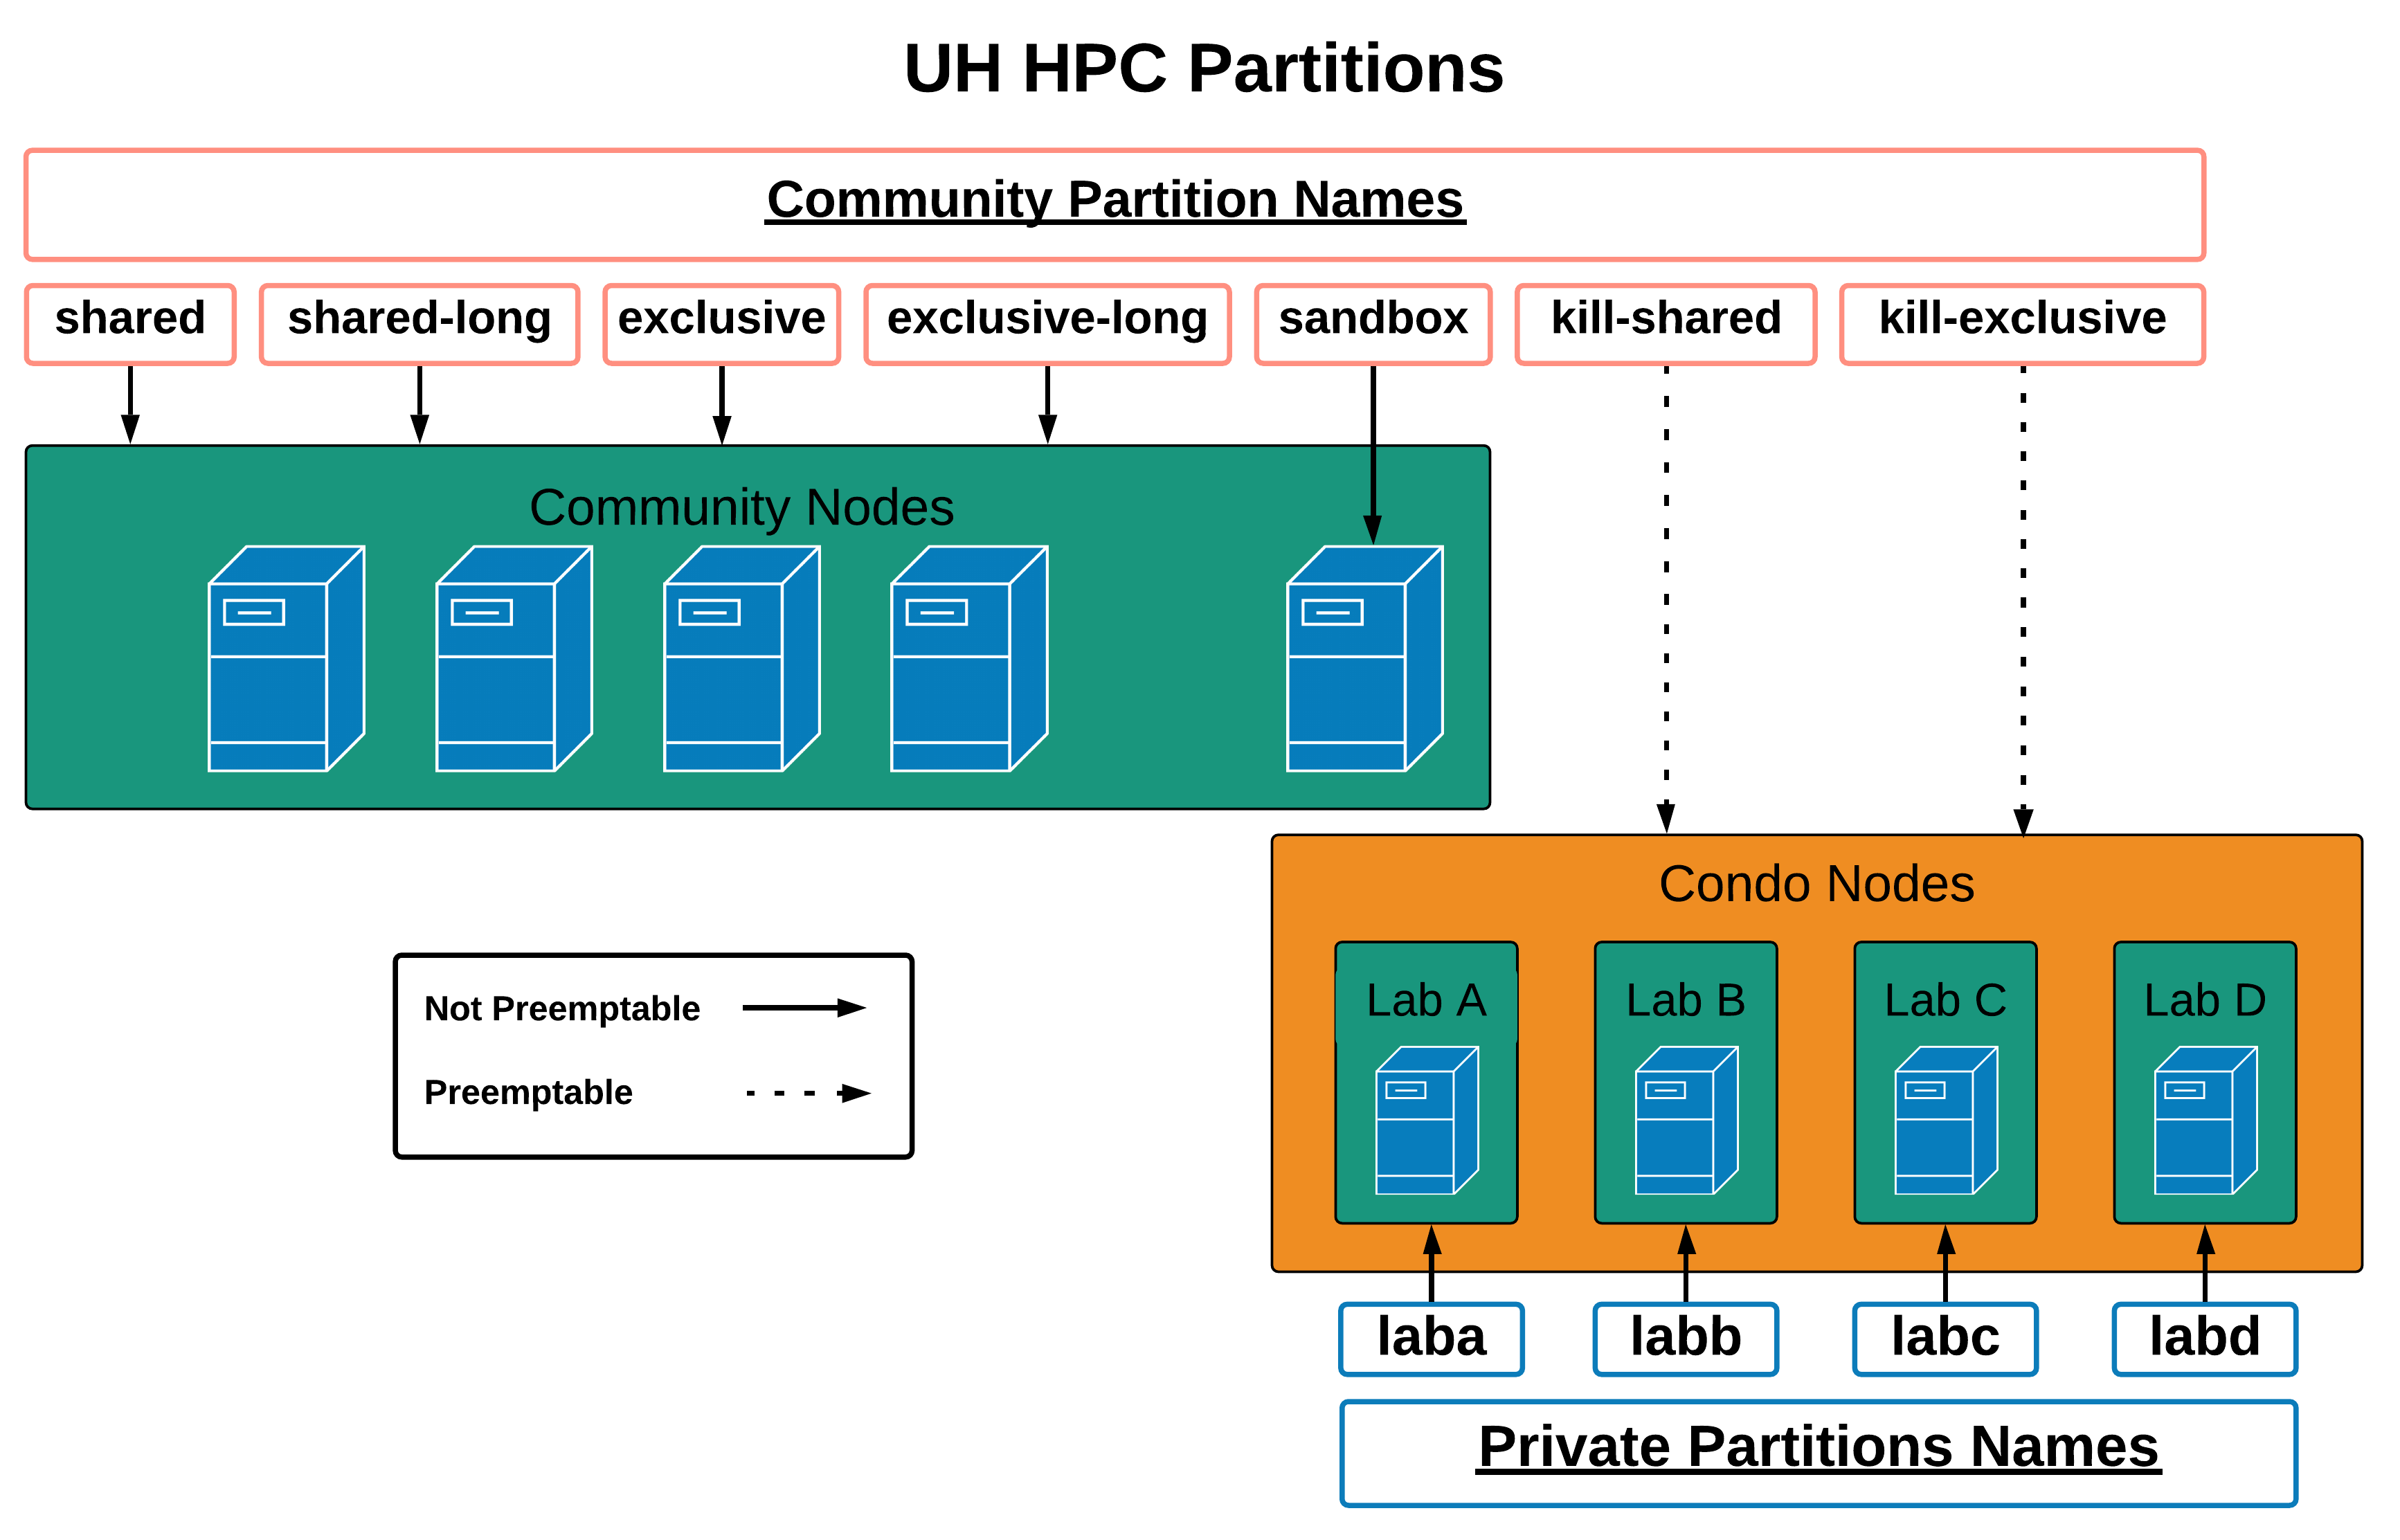
\includegraphics[scale=0.35]{partitions.png}
\end{center}
\end{frame}


\begin{frame}
\footnotesize
\frametitle{Partitions }
\vspace{-10pt}
\begin{block}{\small Details}
\centering
  \resizebox{0.95\textwidth}{!}{%
\begin{tabular}{l || c || c || c || c || c || c }
\toprule                                                                    
\thead{\textbf{Partition}} & \thead{\textbf{Max walltime}} & \thead{\textbf{Jobs - total(running)}} & \thead{\textbf{Max nodes per job}} & \thead{\textbf{Default memory}}& \thead{\textbf{Shared}} & \thead{\textbf{Preemption}}  \\
%\toprule                                                                    
%\toprule                                                                    
\midrule
\midrule
gpu & 3-00:00:00 & $\infty$ & 1 & 512 MB & YES & NO \\
\hline
\hline
gpu-sandbox & 0-04:00:00 & $\infty$(2) & 2 & 512 MB & YES & NO \\
\hline
\hline
sandbox & 0-04:00:00 & $\infty$(2) & 2 & 512 MB & YES & NO \\
\hline
\hline
shared & 3-00:00:00 & $\infty$ & 1 & 512 MB & YES & NO \\
\hline
\hline
shared-long & 7-00:00:00 & 5(2) & 1 & 512 MB & YES & NO \\
\hline
\hline
exclusive & 3-00:00:00 & $\infty$ & 20 & $\infty$ & NO & NO \\
\hline
\hline
exclusive-long & 7-00:00:00 & 5(2) & 20 & $\infty$ & NO & NO \\
\hline
\hline
kill-shared & 3-00:00:00 & $\infty$ & 1 & 512 MB & YES & YES \\
\hline
\hline
kill-exclusive & 3-00:00:00 & $\infty$ & 20 & $\infty$ & NO & YES \\
\bottomrule 
\end{tabular}   
  }

\end{block}

%\vspace{-5pt}
%
%\begin{block}{\small Node Breakdown}
%\centering
  %\resizebox{0.95\textwidth}{!}{%
%\begin{tabular}{l || c || c || c || c || c || c }
%\toprule  
%\thead{\textbf{Partition}} & \thead{\textbf{Intel x86}}  & \thead{\textbf{GPU}} & \thead{\textbf{IB}} & \thead{\textbf{Ethernet}} & \thead{\textbf{Min:Max Cores per node}} & \thead{\textbf{Min:Max Memory per node}\\\textbf{\tiny{(95\% useable)}}} \\
%%\toprule                                                                    
%%\toprule                                                                    
%\midrule
%\midrule
%sandbox & 4 & 0 & 4 & 0 & 20:20 & 128:128 GB \\
%\hline
%\hline
%shared & 152 & 1 & 152 & 0 & 20:40 & 128:1024 GB \\
%\hline
%\hline
%shared-long & 152 & 1 & 152 & 0 & 20:40 & 128:1024 GB \\
%\hline
%\hline
%exclusive & 152 & 1 & 152 & 0 & 20:40 & 128:1024 GB \\
%\hline
%\hline
%exclusive-long & 152 & 1 & 152 & 0 & 20:40 & 128:1024 GB \\
%\hline
%\hline
%kill & 141 & 9 & 133 & 8 & 20:40 & 96:1024 GB \\
%\hline
%\hline
%kill-exclusive & 141 & 9 & 133 & 8 & 20:40 & 96:1024 GB \\
%\bottomrule 
%\end{tabular}   
%}
%
%\end{block}
\end{frame}

\subsection{Constraints \& General Resources}

\begin{frame}
\frametitle{Constraints, General Resources \& Core Specialization}
\vspace{-8pt}
\begin{block}{{\ddash}constraint} Users can select nodes for a job by specifying a value or values for the constraint option. Only nodes having features matching the job constraints will be used to satisfy the request. Multiple constraints may be specified with ``\&'' (AND), ``|'' (OR), etc.
\end{block}
\vspace{-5pt}
\begin{block}{{\ddash}gres} Specifies a comma delimited list of generic consumable resources which a job should be granted access to. 
\end{block}
\vspace{-5pt}
\begin{block}{{\ddash}core-spec}
On {\mana}, the scheduler by default withholds 1 core per node from use by users through a feature in Slurm known as \textbf{core specialization}.  This is done to improve job performance.  This can be overridden by users but is not recommended.
\footnote[1,frame]{\tiny \href{https://slurm.schedmd.com/core_spec.html}{https://slurm.schedmd.com/core\_spec.html}} \footnote[2,frame]{\tiny \href{https://slurm.schedmd.com/SUG14/process_isolation.pdf}{https://slurm.schedmd.com/SUG14/process\_isolation.pdf}}
\end{block}
  \numlessfootnotetxt{\tiny \href{http://go.hawaii.edu/ex2}{Information on Constraints, general resources and node specifications}}
\end{frame}

\part{High Level View of Policies}
\begin{frame}
			 \partpage
\end{frame}

%\section[Resource and Data Governance Policies]{Resource and Data Governance Policies}

%% \begin{frame}
%% 	\frametitle{Overview}
%% 	\begin{itemize}
%% 		\item Login node usage policy
%% 		\item Scratch filesystem purge policy
%% 	\end{itemize}
%% \end{frame}

\section[UH Policies]{UH Policies}
\begin{frame}
  \frametitle{UH Policies}
	\begin{block}{Chapter 708, Hawaii Revised Statutes}
	\begin{itemize}
	\item Access only by authorized people
	\item Should not be used in the act of committing a crime
	\end{itemize}
	\end{block}
	\begin{block}{University of Hawaii Executive Policy E2.210} 
	\begin{itemize}
	\item Protect your password (we will never ask or require your password)
	\item Computer resources should not be used to test or compromise systems without prior authorization
	\item University resources are intended to be used for institutional purposes and may not be used for private gain
	\end{itemize}
	\end{block}
\end{frame}

\section[UH-HPC Usage Policies]{UH-HPC Usage Policies}

\subsection{Login nodes \& DTN nodes}
\begin{frame}
\frametitle{Login nodes \& DTN nodes}
\begin{block}{}
The following actions are acceptable on the shared systems in the UH-HPC:
\begin{enumerate}
\item File/Directory management [ Login \& DTN nodes ]
\item Text editing with a text editor: vi/vim, emacs, nano [ Login \& DTN nodes ]
\item Transferring files to and from the cluster (scp, rsync, SFTP, globus, aspera, lftp, etc.) [ Login \& DTN nodes ]
\item Shall be used to submit batch and interactive jobs [Login nodes]
\item SSH shell access [ Login \& DTN nodes ]
\end{enumerate}
\end{block}

\begin{block}{}
All other action shall take place on a compute node using an interactive session.  
If any actions outside of the sanctioned activities are detected, the following escalation will take place:
\begin{enumerate}
\item The process will be killed without notice
\item If the user continues this action, we will notify the user of violating the policy
\item If the user continues to ignore our warnings, the user may be banned from the cluster for a duration of time
\end{enumerate}
\end{block}
\end{frame}

\subsection{Storage Policy}
\begin{frame}
\frametitle{Storage Policy}
\begin{enumerate}
\item ITS is not responsible for any data that is deleted or loss due to user error, hardware failure, administrator error.  Users are responsible for their own data and are highly encouraged to backup data that is important to them at other storage locations
\item Files located on the scratch file systems are subject to a \textbf{10 day} purge policy that is based on the file/directory modified timestamp.  \textbf{Files that are purge cannot be recovered}.  Users are encouraged to copy their results off the scratch file system as soon as possible upon completion of their job
\item  Home storage currently snapshots once a day per user in case of accidental file deletion
\end{enumerate}
\end{frame}
%\btVFill
%\begin{center}
%\footnotesize \textbf{\emph{Login node usage policy is subject to change~\\Users will be notified via email prior to changes taking effect}}
%\end{center}


\subsection{User Account Life Cycle}
\begin{frame}
\frametitle{User Account Life Cycle}
\begin{enumerate}
\item Accounts that are idle for 120 days will be locked
\item Accounts that have been locked can be unlocked upon request with no further action then emailing us a request to unlock their account
\item Accounts that are idle for a total of 180 days will be purged from the cluster
\item Users that have been purged may request a reactivation of their account, but may be required to take a quiz to confirm retention of how to use the UH-HPC
\item Users that become \textbf{Ohana} (graduated or no longer affiliated with UH) will be allowed up to one year on the UH-HPC before their accounts will be purged  
\item Ohana accounts can be purged sooner based on:
\begin{itemize}
\item Standard idle lockout/purge policy   
\item A faculty or staff requesting a graduated student's account be removed sooner than the one year grace period
\end{itemize}
\item Potential users whom are UH Ohana at the time of account request/creation may not have an account created on the UH-HPC without confirmation from an active faculty member or staff
\end{enumerate}
\end{frame}


\begin{frame}
\frametitle{Where to find all UH-HPC specific policies}
\begin{enumerate}
%\item \href{http://www.hawaii.edu/infotech/policies/itpolicy.html\#appendixa}{Chapter 708, Hawaii Revised Statutes}
%\item \href{http://www.hawaii.edu/infotech/policies/itpolicy.html}{University of Hawaii Executive Policy E2.210}
\item \href{http://go.hawaii.edu/GSY}{Common systems \& Storage}
\item \href{http://go.hawaii.edu/0SG}{User Account life cycle}
\item \href{http://go.hawaii.edu/WSG}{Security}
\item \href{http://go.hawaii.edu/YKG}{For lease storage}
\item \href{http://go.hawaii.edu/GK0}{Condo Program \& Off Warranty condo nodes}
%% \item \href{https://docs.google.com/document/d/1mGcCAsmzGT_hWXLcUNfT2LUwiggCnhqrln32k0IGZZI/}{Special allocations}
\end{enumerate}
\end{frame}
%
%\begin{frame}
%\frametitle{Login Node Usage Policy}\footnotesize
%The login nodes are a shared resource and are the only access to the cluster for hundreds of user and are meant to provide the following functionality for all users: 
%\begin{itemize}
%\item Providing ssh shell access 
%\item Facilitate the transfer files to and from the cluster:\\Globus, sftp, scp, rsync
%\item Launching and monitoring SLURM jobs (batch and interactive)
%\item Modifying text files with a text editor: vi/vim, emacs, nano
%\end{itemize}
%\bigskip
%\begin{itemize}
%\item[--] If we identify or are notified that a user is running computation on the login nodes, the application will be killed
%\item[--] If we determine that a user repeatedly violates the login node policy, even after being warned, the repeat offender can have their cluster account disabled
%\end{itemize}
%\btVFill
%\begin{center}
%\footnotesize \textbf{\emph{Login node usage policy is subject to change~\\Users will be notified via email prior to changes taking effect}}
%\end{center}
%\end{frame}
%
%
%\subsection{Lustre Filesystem Purge Policies}
%\begin{frame}
%\frametitle{{\lustre} Filesystem Purge Policies}
%Due to users not having any quotas on the {\lustre} filesystem, we need some policy in place which removes older files from the system.  To accomplish this, we have implemented a purge policy.
%
%\begin{itemize}
%\item What in \ctilde/lus/ is subject to the purge policy?
   %\begin{itemize}
   %\item \textbf{Answer:} Everything but directories.
   %\end{itemize}
%\item When will my files be purged?
  %\begin{itemize}  
    %\item \textbf{Answer:} Files greater than or equal to 1 Megabyte in size or are empty (0 bytes) that are 35 days old
    %\item \textbf{Answer:} Files between 1 byte and 1 Megabyte in size that are 120 days old
  %\end{itemize}
%\item What is the age based on?
   %\begin{itemize}
   %\item \textbf{Answer:} Age of file is based on creation time
   %\end{itemize}
   %
%%\item How frequently are files for purged?
%%   \begin{itemize}
%%   \item \textbf{Answer:} Taking into account the fill rate of the {\lustre} filesystem, a purge is performend as usage approaches 80\%.
%%   \end{itemize}
%\end{itemize}
%\btVFill
%\begin{center}
%\footnotesize \textbf{\emph{Purge policy is subject to change~\\Users will be notified via email prior to changes taking effect}}
%\end{center}
%\end{frame}
%
%
%
%\begin{frame}
  %\frametitle{How to check file age for purge}
  %A tool is available on the cluster called age\_check.  This tool will list all files that are older than the defined date you set.
%\begin{semiverbatim}\tiny \texttt
  %$[$root@login-0001 \ctilde$]$\$ age\_check -h
  %
  %Usage:
  %age\_check [-s] [-z] [-d] [-f] [-a <age cutoff>] [-p <path]
%
%
  %Options:
%
  %-s -- Sort output
  %
  %-d -- display creation date per file
  %
  %-z -- display size in bytes per file
  %
  %-f -- Do not exclude files between 1 byte and 1 MB
  %
  %-a age -- Lists files that were created at least age days ago (default is 20 days)
  %
  %-p path -- Directory to check in (default is /lus/scratch/root)
%
  %
  %Example:
  %age\_check -a 30  
%
%\end{semiverbatim}
%
%\end{frame}
   

%\part{Data Governance \& Security}
\begin{frame}
			 \partpage
\end{frame}

\section[Data Governance]{Data Governance}

\begin{frame}
  \frametitle{What is data governance}
  %        \begin{definition}\footnotesize
  %          Data governance is a data management concept concerning the capability that enables an organization to ensure that high data quality exists throughout the complete lifecycle of the data. The key focus areas of data governance include availability, usability, consistency, data integrity and data security and includes establishing processes to ensure effective data management throughout the enterprise such as accountability for the adverse effects of poor data quality and ensuring that the data which an enterprise has can be used by the entire organization.
  %        \footnote[1,frame]{\tiny \href{https://en.wikipedia.org/wiki/Data\_governance}{https://en.wikipedia.org/wiki/Data\_governance}}
  %        \end{definition}
  \begin{itemize}
  \item Defines how data is collected, stored, and used
  \item Defines who can access data, when, and under what conditions
  \item Establishes decision rights
  \item Establishes clear lines of accountability
  \item Gives a voice to all appropriate parties
  \item Provides a mechanism for conflict resolutions involving data
  \end{itemize}
\end{frame}


\begin{frame}
  \frametitle{Goals of data governance @ UH}
  \begin{block}{}
    \href{https://www.hawaii.edu/offices/vp-academic-planning-policy/uh-institutional-data-governance/}{The Data Governance Office at the University of {\hawaii}} creates policies and procedures focused on the privacy and security of data under the University’s care. 
  \end{block}
  \begin{block}{Goals}
  \begin{itemize}
  \item Protect the privacy and security of ``Protected Data''
    \begin{itemize}
    \item All non-public data
    \item Institutional data
    \item Research data
    \end{itemize}
%  \item Produce higher quality data for informed decision making
  \item Promote efficient use of resources
  \item Increase transparency and accountability
  \end{itemize}
  \end{block}
\end{frame}


\subsection{Data Classifications @ UH}
\begin{frame}
  \frametitle{Data Classifications @ UH}
  \vspace{-5pt}
  \makebox[\linewidth][c]{
    \resizebox{\textwidth}{!}{%
      \begin{tabular}{l||p{6cm}||p{6cm}}
      %  \multicolumn{8}{c}{ {\large {\textbf{UH-HPC Resource Summary} } } } \\ 
	\toprule                                                                    
        \thead{\large\textbf{Category}} & \thead{\large\textbf{Definition}} & \thead{\large\textbf{Examples}} \\ 
	\midrule  \midrule %\hline
        \textbf{Public} & Access is not restricted and is subject to open records requests  & Student directory information, employee’s business contact info \\
	\midrule  \midrule %\hline
        \multicolumn{3}{c}{ {\large {\textbf{Protected Data} } } } \\ 
	\midrule  \midrule %\hline
        \textbf{Restricted} & Used for UH business only; will not be distributed to external parties; released externally only under the terms of a written MOA or contract & Student contact information, UH ID number \\
	\midrule  
        \textbf{Sensitive} & Data subject to privacy considerations  & Date of birth, job applicant records, salary/payroll information, most student information \\
	\midrule  
        \textbf{Regulated} & Inadvertent disclosure or inappropriate access requires a breach notification by law or is subject to financial fines & FN or first initial/LN in combination with SSN, driver license number, or bank information; credit card, HIPAA, or financial aid information \\            
    \bottomrule
      \end{tabular}%
    }    }
  \vfill
  \centering
    The \href{https://datagov.intranet.hawaii.edu/dgp/}{Data Governance Process (DGP)} applies to collecting, managing, sharing or using data that can be classified as protected data
\end{frame}  

\section{Regulations}

\begin{frame}
  \frametitle{Regulations}
\begin{block}{}
  The following lists of regulations are not exahustive lists that may apply to your data at the university (personal \& research).
  It is important that you know and understand what regulations the data you are working with is subject to.

\end{block}
\end{frame}

\subsection{Personally Identifiable Information (PII)  \& Financial Regulations}
\begin{frame}
  \frametitle{Regulations}
  \begin{block}{Personally Identifiable Information (PII)  \& Financial Regulations}
    \begin{itemize}
    \item \href{https://studentprivacy.ed.gov/ferpa-regulations}{Family Educational Rights and Privacy Act (FERPA)} [UH Policy \href{https://www.hawaii.edu/policy/?action=viewPolicy\&policySection=ap\&policyChapter=7\&policyNumber=022\&menuView=closed}{AP 7.022}]
      \begin{itemize}
      \item Federal law that protects the privacy of student education records
      \end{itemize}
    
    \item Higher Education Act (HEA)
      \begin{itemize}
      \item Federal law that protects the federal financial aid information
      \end{itemize}
      
    \item \href{https://www.ftc.gov/tips-advice/business-center/privacy-and-security/gramm-leach-bliley-act}{Gramm-Leach-Bliley Act (GLBA)}
      \begin{itemize}
      \item Federal law that requires finanical institutions to explain how they share \& protect customer's data
      \end{itemize}

    \item \href{https://gdpr-info.eu/}{General Data Protection Regulation (GDPR)}
      \begin{itemize}
      \item A European Union (EU) consumer protection law that applies to companies collecting PII as part of delivering goods and services
      \end{itemize}

    \item \href{https://www.hhs.gov/hipaa/for-professionals/security/laws-regulations/index.html}{Health Insurance Portability and Accountability Act (HIPPA}) [UH Policy \href{https://www.hawaii.edu/policy/index.php?action=viewPolicy\&policySection=ep\&policyChapter=2\&policyNumber=217\&menuView=closed}{EP 2.217}]
      \begin{itemize}
      \item Federal law that protects the privacy of health information
        \item \href{https://www.hawaii.edu/infosec/hipaa/}{HIPPA @ UH}
      \end{itemize}
    \end{itemize}  
  \end{block}
\end{frame}  



\subsection{Federal Regulations}
\begin{frame}
  \frametitle{Regulations}
  \vspace{-5pt}
  \begin{block}{Federal Regulations}
    \begin{itemize}
    \item \href{https://csrc.nist.gov/publications/detail/sp/800-171/rev-1/final}{National Institute of Standards and Technology Special Programs (NIST) 800-171}
      \begin{itemize}
      \item Federal Department of Defense (DoD) standards aimed at safeguarding Controlled Unclassified Information (CUI)
      \item May apply to grants from DoD and possibly other federal agencies
      \end{itemize}
    
    \item \href{https://www.hsdl.org/?abstract\&did=461297}{National Industrial Security Program [DoD Directive 5220.22-M]}
      \begin{itemize}
      \item Classified data subject to regulation
      \end{itemize}
      
    \item \href{https://www.pmddtc.state.gov/ddtc_public?id=ddtc_public_portal_itar_landing\#tab-itar}{Export Control \& International Traffic in Arms Regulations (ITAR)}
      \begin{itemize}
      \item Federal regulations that impose access, dissemination or participation restrictions on the use and/or transfer of commodities, technical data, or the provision of services subject to United States (US) export controls for reasons of national security, foreign policy, anti-terrorism or non-proliferation
      \end{itemize}

    \item \href{https://www.bis.doc.gov/index.php/regulations/export-administration-regulations-ear}{Export Administration Regulations (EAR)}
      \begin{itemize}
      \item EAR govern whether a person may export a thing from the U.S., reexport the thing from a foreign country, or transfer a thing from one person to another in a foreign country. The EAR apply to physical things (sometimes referred to as "commodities") as well as technology and software.\footnote{\label{EAR on Wikipedia}\tiny\url{https://en.wikipedia.org/wiki/Export_Administration_Regulations}} 
      \end{itemize}
    \end{itemize}
\end{block}
\end{frame}  


\subsection{State Regulations}
\begin{frame}
  \frametitle{Regulations}
  \vspace{-5pt}
  \begin{block}{State Regulations}
    \begin{itemize}
    \item \href{https://www.capitol.hawaii.gov/hrscurrent/Vol11_Ch0476-0490/HRS0487N/HRS_0487N-.htm}{{\hawaii} Revised Statues (HRS) 487N}
      \begin{itemize}
      \item State law that defines the breach notification to the legislature
      \item Examples: First name or First initial and Last name in combination with at least one of the following
        \begin{itemize}
        \item Social Security Number (SSN)
        \item Driver license or State ID \#
        \item Person's finanical account information
          \end{itemize}
      \end{itemize}
    
    \item \href{https://www.capitol.hawaii.gov/hrscurrent/Vol02_Ch0046-0115/HRS0092F/HRS_0092F-.htm}{Uniform Information Practices Act (UIPA)[HRS Chapter 92F]}
      \begin{itemize}
      \item Governs open records requests
      \end{itemize}
    \end{itemize}
\end{block}
\end{frame}  




\subsection{UH Data Related Policies \& Procedures}
\begin{frame}
  \frametitle{UH Data Related Policies \& Procedures}
  \vspace{-7pt}
\makebox[\linewidth][c]{
    \resizebox{\textwidth}{!}{%                                                                                                                                                                                                                                                       
      \begin{tabular}{l||l}
      %  \multicolumn{8}{c}{ {\large {\textbf{UH-HPC Resource Summary} } } } \\                                                                                                                                                                                                       
        \toprule
        \thead{\large\textbf{Policy}} & \thead{\large\textbf{Description}} \\
        \midrule  \midrule %\hline
        \multicolumn{2}{c}{ {\large {\textbf{Administrative Procedure} } } } \\  
        \midrule \midrule
        \href{https://www.hawaii.edu/policy/?action=viewPolicy\&policySection=ap\&policyChapter=2\&policyNumber=215\&menuView=closed}{\textbf{AP2.215}} & Mandatory Training \& Continuing Education Requirements \\
        \midrule
        \href{https://www.hawaii.edu/policy/?action=viewPolicy\&policySection=ap\&policyChapter=7\&policyNumber=022\&menuView=closed}{\textbf{AP7.022}} & FERPA \\
        \midrule \midrule
        \multicolumn{2}{c}{ {\large {\textbf{Executive Policy} } } } \\  
        \midrule \midrule
        \href{https://www.hawaii.edu/policy/?action=viewPolicy\&policySection=ep\&policyChapter=2\&policyNumber=210\&menuView=closed}{\textbf{EP2.210}} & Use and Management of Information Technology Resources \\
        \midrule
        \href{https://www.hawaii.edu/policy/?action=viewPolicy\&policySection=ep\&policyChapter=2\&policyNumber=213\&menuView=closed}{\textbf{EP2.213}} & System and Campus Wide Electronic Channels for Communicating with Students\\
        \midrule        
        \href{https://www.hawaii.edu/policy/?action=viewPolicy\&policySection=ep\&policyChapter=2\&policyNumber=214\&menuView=closed}{\textbf{EP2.214}} & Data Classification Categories \& Information Security Guidelines \\
        \midrule
        \href{https://www.hawaii.edu/policy/?action=viewPolicy\&policySection=ep\&policyChapter=2\&policyNumber=215\&menuView=closed}{\textbf{EP2.215}} & Institutional Data Governance \\
        \midrule
        \href{https://www.hawaii.edu/policy/?action=viewPolicy\&policySection=ep\&policyChapter=2\&policyNumber=216\&menuView=closed}{\textbf{EP2.216}} & Institutional Records Management \& Electronic Approvals/Signatures (\textit{Pending Approval}) \\
        \midrule
        \href{https://www.hawaii.edu/policy/?action=viewPolicy\&policySection=ep\&policyChapter=2\&policyNumber=217\&menuView=closed}{\textbf{EP2.217}} & HIPPA (\textit{To be Revised}) \\
        \midrule
        \href{https://www.hawaii.edu/policy/?action=viewPolicy\&policySection=ep\&policyChapter=2\&policyNumber=218\&menuView=closed}{\textbf{EP2.218}} & Online Approvals of Internal University Transactions\\
        \midrule
        \textbf{EP2.2xx} & Student Online Data Protection Requirements (\textit{Draft}) \\
        \midrule
        \href{https://www.hawaii.edu/policy/?action=viewPolicy\&policySection=ep\&policyChapter=2\&policyNumber=215\&menuView=closed}{\textbf{EP2.215}} & Institutional Data Governance \\
        \midrule
        \href{https://www.hawaii.edu/policy/?action=viewPolicy\&policySection=ep\&policyChapter=8\&policyNumber=200\&menuView=closed}{\textbf{EP8.200}} & Policy on Contracts \& Signing Authority \\
        \bottomrule
      \end{tabular}%
      }
}
\vspace{-5pt}


\end{frame}  



\section[Security]{Security}


\subsection{Information Security Program}
\begin{frame}
  \frametitle{Information Security Program}

  The \href{https://www.hawaii.edu/infosec/infosecprogram/}{University of {\hawaii} Information Security Program} is comprised of the following strategic areas:

  \begin{block}{Strategic Areas}
    \begin{itemize}
  \item Data Governance \& Oversight
  \item Information Security Audits \& Risk Assessments
  \item Information Security Policies \& Procedures
  \item Identity Management \& Access Controls
  \item Information Security Training \& Awareness
  \end{itemize}
  \end{block}
\end{frame}  


\subsection{Data Protection}
\begin{frame}
  \frametitle{Protect Your Data!}
  \vspace{-10pt}
  \begin{block}{Know which files have sensitive information}
    \begin{itemize}
    \item Use \href{http://www.hawaii.edu/askus/1297}{Spirion} (formerly Identity Finder) to scan for sensitive information
    \end{itemize}
  \end{block}
  \vspace{-3pt}  
  \begin{block}{Protect sensitive/regulated data as required by UH policy}
  \begin{itemize}
  \item UH Policy \href{https://www.hawaii.edu/policy/EP2.214}{EP 2.214}
  \end{itemize}
  \end{block}
  \vspace{-3pt}  
  \begin{block}{Data protection life cycle}
    \begin{itemize}
    \item Back up your data regularly
    \item Transmit and share sensitive data in a secure manner, e.g., SFTP, \href{https://www.hawaii.edu/filedrop/}{UH FileDrop}
    \item Protect sensitive/regulared data with encryption
    \item Securely delete any sensitive data that is no longer needed
    \end{itemize}
  \end{block}    
  \vspace{-3pt}  
  \begin{block}{Physical Security of data repository with sensitive data}
    \begin{itemize}
    \item Paper documents should be stored in a secured location, not accessible by unauthorized individuals e.g., a locked file cabinent
    \item External hard drives should be stored in a secured location e.g., a locked file cabinent
    \end{itemize}
  \end{block}    
\end{frame}  

\subsection{Device Protection}
\begin{frame}
  \frametitle{Protect Your Computers!}
  \begin{block}{Operating System (OS) }
    \begin{itemize}
    \item Apply updates to your OS and applications frequently and on a regular basis
    \end{itemize}
  \end{block}

  \begin{block}{Protective Software}
  \begin{itemize}
  \item Install and keep up to date protective software such as \href{http://www.hawaii.edu/askus/1254}{anti-virus}
  \end{itemize}
  \end{block}

  \begin{block}{Physical Access}
    \begin{itemize}
    \item Never leave your devices logged-in \& unattended
    \item Control physical access to your machines
    \item When you step away from your machine, lock your screen
    \item Require password authentication when unlocking or accessing your machine
    \end{itemize}
  \end{block}    
\end{frame}  


\subsection{Storing and transmitting data with Google products}
\begin{frame}
  \frametitle{Storing and transmitting data with Google products}
  \onslide<1->{\begin{block}{Question}
    \begin{columns}[T ]
      \begin{column}{0.15\textwidth}\hfill
\includegraphics[scale=0.05]{question_mark.png}\end{column}
      \begin{column}{0.80\textwidth}
        Is it safe to store and transmit sensitive or regulated data using the different Google products offerred at the University?
        e.g., Google Docs, Google Drive, Gmail
      \end{column}
    \end{columns}
    \end{block}
    }
  \vfill
  \onslide<2->{\begin{block}{Answer}
%https://www.kissclipart.com/stop-hand-clipart-stop-sign-clip-art-pgay2w/
\begin{columns}
\begin{column}{0.15\textwidth}\hfill\includegraphics[scale=0.05]{stop_hand.png}\end{column}
\begin{column}{0.70\textwidth}
    \centering
    {\HUGE \textbf{\textit{NO!}}}\Large~\\Do \textbf{NOT} store or transmit sensitive or regulated information in \emph{Google Docs}, \emph{Google Drive} or \emph{Email}~\\~\\Use the \href{https://www.hawaii.edu/filedrop/}{UH FileDrop} to securely transmit files under 1000 megabytes inside
\end{column}
\begin{column}{0.15\textwidth}\includegraphics[scale=0.05]{stop_hand.png}\end{column}
\end{columns}
    \end{block}}
\end{frame}



\subsection{Account protection}
\begin{frame}
  \frametitle{Protect Your Account!}
\begin{columns}
\begin{column}{0.45\textwidth}
\begin{block}{}
  \begin{itemize}
  \item User strong passwords and a strong password management strategy
  \item \textbf{DO NOT RE-USE PASSWORDS!}
  \item Consider using a passphrase
    \begin{itemize}
    \item lower/uppercase
    \item numbers
    \item special characters
    \item character substitutions, e.g.,
      \begin{itemize}
      \item o $\Longrightarrow$ 0
      \item a $\Longrightarrow$ @
      \item i $\Longrightarrow$ 1
      \end{itemize}
    \end{itemize}
  \item Check your password strength: \href{https://lastpass.com/howsecure.php}{https://lastpass.com/howsecure.php}
  \item Monitor your accounts for suspicious activity
  \end{itemize}
  \end{block}
\end{column}
\begin{column}{0.49\textwidth}
\begin{block}{}
  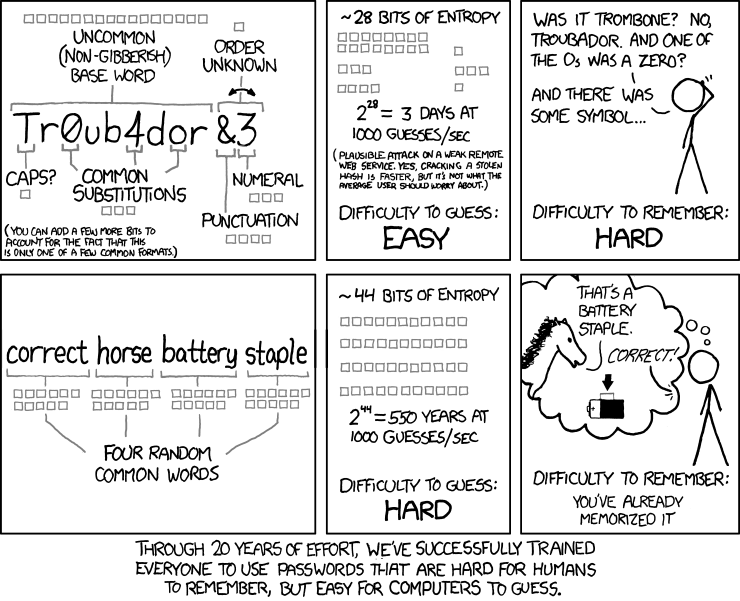
\includegraphics[scale=0.25]{password_strength.png}
  \numlessfootnotetxt{\label{xkcd_pasword_strnght}\tiny\url{https://xkcd.com/936/}}
\end{block}
\end{column}
\end{columns}
\end{frame}  


\section*{More Information}
\begin{frame}
  \frametitle{More Information}
  You can find more information about Data Governance and Security at UH at the following links:
  \begin{itemize}
  \item \href{https://datagov.intranet.hawaii.edu/}{Data Governance internal site}
  \item \href{https://datagov.intranet.hawaii.edu/training/}{Data Governance \& Security trainings/presentations}
  \item \href{https://datagov.intranet.hawaii.edu/institutional-data-classification-levels/}{Institutional data classifications}
  \item \href{https://www.hawaii.edu/infosec/}{Information Security (InfoSec) at UH}
  \item \href{https://www.hawaii.edu/its/alerts/}{Security notices and other alerts from UH Information Technology Services (ITS)}
  \item \href{https://www.hawaii.edu/its/itacw/}{IT All Campus Workshop \ddash Yearly during the summer}
  \end{itemize}
\end{frame}  




  %% \item General Data Protection Regulation (GDPR)
  %%   \begin{itemize}
  %%   \item A European Union (EU) consumer protection law that applies to companies collecting personally identifiable information (PII) as part of delivering goods and services
  %%   \end{itemize}

  %% \item General Data Protection Regulation (GDPR)
  %%   \begin{itemize}
  %%   \item A European Union (EU) consumer protection law that applies to companies collecting personally identifiable information (PII) as part of delivering goods and services
  %%   \end{itemize}

  %% \item General Data Protection Regulation (GDPR)
  %%   \begin{itemize}
  %%   \item A European Union (EU) consumer protection law that applies to companies collecting personally identifiable information (PII) as part of delivering goods and services
  %%   \end{itemize}

  %% \item General Data Protection Regulation (GDPR)
  %%   \begin{itemize}
  %%   \item A European Union (EU) consumer protection law that applies to companies collecting personally identifiable information (PII) as part of delivering goods and services
  %%   \end{itemize}

    
  %% \end{itemize}
  
  %% \begin{table}
  %%   \centering
  %%   \resizebox{\textwidth}{!}{%
  %%     \begin{tabular}{l||p{6cm}||p{6cm}}
  %%     %  \multicolumn{8}{c}{ {\large {\textbf{UH-HPC Resource Summary} } } } \\ 
  %%       \toprule                                                                    
  %%       \thead{\large\textbf{Regulation}} & \thead{\large\textbf{Description}} & \thead{\large\textbf{}} \\ 
  %%       \midrule  \midrule %\hline
  %%       \textbf{Public} & Access is not restricted and is subject to open records requests  & Student directory information, employee’s business contact info \\
  %%       \midrule  \midrule %\hline
  %%       \multicolumn{3}{c}{ {\large {\textbf{Protected Data} } } } \\ 
  %%       \midrule  \midrule %\hline
  %%       \textbf{Restricted} & Used for UH business only; will not be distributed to external parties; released externally only under the terms of a written MOA or contract & Student contact information, UH ID number \\
  %%       \midrule  
  %%       \textbf{Sensitive} & Data subject to privacy considerations  & Date of birth, job applicant records, salary/payroll information, most student information \\
  %%       \midrule  
  %%       \textbf{Regulated} & Inadvertent disclosure or inappropriate access requires a breach notification by law or is subject to financial fines & FN or first initial/LN in combination with SSN, driver license number, or bank information; credit card, HIPAA, or financial aid information \\            
  %%   \bottomrule
  %%     \end{tabular}%
  %%   }
  %% \end{table}


%% \begin{columns}
	%% \begin{column}{0.46\textwidth}
	%% 	\begin{block}{}
	%% 	\begin{itemize}
	%% 		\item Quad Data Rate (QDR)\\InfiniBand{\regtrademark} (IB)   
	%% 			\begin{itemize}
	%% 				\item 40 Gbit
	%% 				\item Older compute nodes
	%% 				\item low latency ($\approx1.3\mu$s)
	%% 				\item non-blocking
	%% 			\end{itemize}
	%% 			~\\
	%% 		\item 25/100 Gbit Ethernet
	%% 			\begin{itemize}
	%% 				\item Newer compute nodes
	%% 				\item Nodes connected @ 25~Gbit
	%% 				\item non-blocking
	%% 			\end{itemize}
	%%         \end{itemize}
        %%         \end{block}
	%% \end{column}
	%% \begin{column}{0.46\textwidth}
	%% 	\begin{block}{External Networks}
	%% 	\begin{itemize}
	%% 		\item 100 Gbit SciDMZ
	%% 			\begin{itemize}
	%% 				\item Login \& compute nodes\\connected via a firewall
	%% 				\item DTNs are directly connected
	%% 			\end{itemize}
	%% 	\end{itemize}
        %%         \end{block}
	%% \end{column}
	%% \end{columns}


        



%% \begin{frame}
%% 	\frametitle{Terminology}
%% 	\begin{itemize}
%% 	\item \textbf{Symbolic Link (symlink)} -- A file that contains a reference to another file or directory
%% 	\item \textbf{Command-line interface/interpreter (CLI)} -- A text-based user interface used to view and manage computer files 
%% 	\item \textbf{Message Passing Interface (MPI)} -- A standard that is used by programs to pass messages between nodes
%% 	\item \textbf{High Performance Compute (HPC)} -- A computing paradigm in which applications are typically a tightly coupled parallel job that benefit from a low-latency interconnect
%% 	\item \textbf{High Throughput Compute (HTC)} -- A computing paradigm that focuses on the efficient execution of a large number of loosely-coupled tasks
%%         \item \textbf{Modified time} -- The last time the file was modified (content has been modified)\footnote{\label{Types of timestamps}\tiny\url{https://unix.stackexchange.com/a/2465}}
%%         \item \textbf{Shell script (script)} -- A computer program designed to be run by a CLI\footnote{\label{Shell script}\tiny\url{https://en.wikipedia.org/wiki/Shell_script}}
%% %        \item Pleasantly Parallel -- Processes are independent and no communication is necessary 
%% 	\end{itemize}


%% \end{frame}


%% \section[University of Hawai'i High Performance Compute Cluster]{University of Hawai'i High Performance Compute Cluster}
%% \begin{frame}
%%     \frametitle{University of {\hawaii} High Performance Compute Cluster}
%%     \begin{itemize}
%%     \item The University~of~{\hawaii} High Performance Compute Cluster~({\uhhpc}) is \textbf{free} to use for all active faculty, staff, and students affiliated with the University of {\hawaii}
%%     \item Community acquired nodes are equally accessible to all users
%%     \item Nodes purchased through the {\textbf{condo program}} are shared with the community, but priority is given to the node owner and their agents
%% 		\item Nodes may be {\textbf{leased}} from the community pool
%% 		\item Additional permanent storage can be leased with up to a five year contract by faculty \& staff
%%     \end{itemize}
%% 		\begin{block}{UH-HPC Resource Summary}
%%   \begin{table}
%%     \centering
%%     \resizebox{\textwidth}{!}{%
%%       \begin{tabular}{l||l||l||l||l||l||l||l}
%%       %  \multicolumn{8}{c}{ {\large {\textbf{UH-HPC Resource Summary} } } } \\ 
%% 			\toprule                                                                    

%%               {}               & \thead{\textbf{Nodes}} & \thead{\textbf{CPU Cores}} & \thead{\textbf{Memory}} & \thead{\textbf{GPUs}} & \thead{\textbf{Home/Group Space}} & \thead{\textbf{Scratch Space}} & Storage for lease \\ 
%% 							\midrule  \midrule %\hline
%%         \thead{\textbf{Total}} & 297                    & 6,308                      & 50 TB                   &  56                   & 80 TB                             &  700 TB                        & 1 PB              \\ %\hline
%% 				\bottomrule
%%       \end{tabular}%
%%     }
%%   \end{table}
%% 	\end{block}
%% \end{frame}

%% \subsection{Condo Program \& Leasing}
%% \begin{frame}
%%   \frametitle{What is the Condo Program \& leasing?}
%% 	\begin{block}{Condo Program}\scriptsize
%% 		\begin{itemize}
%% 		\item The condo program allows faculty \& staff to purchase nodes and have them integrated with the UH-HPC
%% 		\item Condo nodes can take advantage of networking and storage infrastructure that one may not typically have access to
%% 		\item Condo nodes are managed and maintained by ITS staff
%% 		\item No maintenance fee will be assessed until the node is off warranty (typically five years)
%% 		\end{itemize}
%% 	\end{block}
%% 	\begin{block}{Leasing}\scriptsize
%% 		\begin{itemize}
%% 		\item Nodes leased from the community can have a contract period from one month, up to one year
%% 		\item Node lessees are provided priority access to their leased hardware
%% 		\item Leases are not considered an equipment purchase
%% 		\end{itemize}
%% 	\end{block}
%% \end{frame}

%% \subsection{Storage}
%% \begin{frame}
%%   \frametitle{Storage}
%%   The UH-HPC has two classes and three types of storage that users can potentially access.\\Each type of storage has their own attributes and restrictions
%% 	\begin{columns}
%% 		\begin{column}{0.46\textwidth}
%% 		\begin{block}{Free Storage}
%% 			\begin{enumerate}
%% 			\item Permanent Storage
%% 				\begin{itemize}
%% 				\item Home Storage
%% 				\item Group/Lab Storage
%% 				\end{itemize}
%% 			\item Scratch Storage
%% 				\begin{itemize}
%% %				\item {\lustre}(TBD)
%% 				\item Network File System (NFS)
%% 				\end{itemize}
%% 		\end{enumerate}
%% 		\end{block}
%% 		\end{column}
%% 		\begin{column}{0.46\textwidth}
%% 		\begin{block}{For Fee Storage}
%% 			\begin{enumerate}
%% 				\item Long Term Storage (LTS)
%% 		\end{enumerate}
%% 		\end{block}
%% 		\end{column}
%% 	\end{columns}      
%% \end{frame}

%% \begin{frame}
%%   \frametitle{Permanent Storage}
%%   \begin{enumerate}
%%   \item Home Storage
%%     \begin{itemize}
%%     \item {\textbf{Purpose}}: Personal storage for applications and active data that needs to persist on the UH-HPC
%%     \end{itemize}
%%   \item Group/Lab Storage
%%     \begin{itemize}
%%     \item {\textbf{Purpose}}: Group/Lab storage allows users to share data \& applications with a need for persistence on the UH-HPC
%%     \end{itemize}
%%   \end{enumerate}
%% ~\\
%%   All permanent storage options on the UH-HPC have the following attributes:
%%   \begin{itemize}
%%   \item 50 GB default quota with a max quota of 300 GB
%%   \item Quota increases are re-evaluated annually
%%   \item Available on all nodes
%%   \item Freely available to users
%%   \end{itemize}

%% \end{frame}


%% \begin{frame}
%%   \frametitle{Scratch Storage}
%%   \begin{enumerate}
%% %    \item {\lustre (TBD)}
%% %      \begin{itemize}
%% %      \item High performance parallel file system 
%% %      \item 50 TB quota
%% %      \end{itemize}
%%     \item NFS
%%       \begin{itemize}
%% %      \item Not a parallel file system
%%       \item 5 TB quota
%%       \end{itemize}
%%   \end{enumerate}
%% ~\\
%%   All scratch file systems on the UH-HPC have the following attributes:
%%   \begin{itemize}
%%   \item \textbf{Purge policy} -- 10 days based on file modify time
%%   \item Available on all nodes
%%   \item Freely available to users
%%   \end{itemize}

%% \end{frame}



%% %\begin{frame}
%%   %\frametitle{For Fee Storage}
%%   %\begin{enumerate}
%%     %\item ValueStorage
%%       %\begin{itemize}
%%       %\item Enterprise class equipment 
%%       %\item 10 Gbit connected to the UH-HPC
%%       %\item Currently only accessible on the DTNs and login nodes
%%       %\end{itemize}
%%     %\item LTS  
%%       %\begin{itemize}
%%       %\item Cheap-n-Deep
%%       %\item 100 Gbit connected to the UH-HPC
%%       %\item Accessible on all nodes
%%       %\end{itemize}
%%   %\end{enumerate}
%% %\end{frame}



%% \subsection{Networking}
%% \begin{frame}
%%   \frametitle{Networking}
%% 	\begin{columns}
%% 	\begin{column}{0.46\textwidth}
%% 		\begin{block}{Internal Networks}
%% 		\begin{itemize}
%% 			\item Quad Data Rate (QDR)\\InfiniBand{\regtrademark} (IB)   
%% 				\begin{itemize}
%% 					\item 40 Gbit
%% 					\item Older compute nodes
%% 					\item low latency ($\approx1.3\mu$s)
%% 					\item non-blocking
%% 				\end{itemize}
%% 				~\\
%% 			\item 25/100 Gbit Ethernet
%% 				\begin{itemize}
%% 					\item Newer compute nodes
%% 					\item Nodes connected @ 25~Gbit
%% 					\item non-blocking
%% 				\end{itemize}
%% 	        \end{itemize}
%%                 \end{block}
%% 	\end{column}
%% 	\begin{column}{0.46\textwidth}
%% 		\begin{block}{External Networks}
%% 		\begin{itemize}
%% 			\item 100 Gbit SciDMZ
%% 				\begin{itemize}
%% 					\item Login \& compute nodes\\connected via a firewall
%% 					\item DTNs are directly connected
%% 				\end{itemize}
%% 		\end{itemize}
%%                 \end{block}
%% 	\end{column}
%% 	\end{columns}
%% \end{frame}



%% \subsection{User Support}
%% \begin{frame}
%%   \frametitle{User Support}

%%   \begin{block}{Online documents \& FAQ}
%%     Users are encouraged to look through the online documentation \& FAQ prior to contacting ITS-CI directly.  Many questions we receive are repeat questions and we try to capture them in our FAQ~\\
%%     \href{https://www.hawaii.edu/its/ci/xcat/}{xCAT cluster information, policies \& FAQ}
%%   \end{block}
%%   \begin{block}{Contact Information}
%%     If your question is not answered in our online documentation, please contact us at: UH-HPC-Help@lists.hawaii.edu
    
%%     \begin{itemize}
%%     \item For batch jobs \ldots
%%       \begin{itemize}
%%       \item[--] Job ID, path to submission script, submission command, error file location, output files
%%       \end{itemize} 
%%     \item For other problems \ldots
%%       \begin{itemize}
%%       \item[--] State the problem, command issued, host, directory, remote host, error messages
%%       \end{itemize}
%%     \end{itemize}
%%   \end{block}
%% \end{frame}



%\section{Problem Reporting}
\begin{frame}
\frametitle{Problem Reporting}
\begin{itemize}
\item Always email UH-HPC-Help@lists.hawaii.edu
\item For batch jobs \ldots
\begin{itemize}
\item[--] Job ID, path to submission script, submission command, error file location, output files
\end{itemize} 
\item For other problems \ldots
\begin{itemize}
\item[--] State the problem, command issued, host, directory, remote host, error messages
\end{itemize}
\end{itemize}
\end{frame}

%\section{Cluster Etiquette}
\begin{frame}
  \frametitle{Cluster Etiquette}
  \begin{itemize}
  \item Never run anything on the login nodes
  \item Try to request only the resources that your job needs.  Leaving unneeded resources available, allows other users to use them
  \item Test your application in an interactive session before scheduling a long running job
    \begin{itemize}
    \item[--] This can help identify what resources your job will require, and potentially aid you in correctly sizing what resources you request.
    \end{itemize}
  \item Use the nodes in the sb.q to validate your slurm script runs as intended
    \begin{itemize}
    \item[--] This helps to reduce the chance of you having a small error that kills your job prematurely after waiting for resources
    \end{itemize}
  \item Always run jobs from within {\ctilde}/lus/ directory to ensure output is written there and does not fill up the system filesystem
  \end{itemize}
\end{frame}

%\section{Policies}
%% \begin{frame}
%% 	\frametitle{Overview}
%% 	\begin{itemize}
%% 		\item Login node usage policy
%% 		\item Scratch filesystem purge policy
%% 	\end{itemize}
%% \end{frame}

\subsection{Use and Management of IT Resources @ UH }
\begin{frame}
  \frametitle{Use and Management of IT Resources @ UH }
  All usage of the {\craycs} must be in compliance with \href{http://www.hawaii.edu/infotech/policies/itpolicy.html\#appendixa}{Chapter 708, Hawaii Revised Statutes} and is subject to University of Hawaii Executive Policy \href{http://www.hawaii.edu/infotech/policies/itpolicy.html}{E2.210}. 
\end{frame}

\subsection{Login Node Usage Policy}
\begin{frame}
\frametitle{Login Node Usage Policy}\footnotesize
The login nodes are a shared resource and are the only access to the cluster for hundreds of user and are meant to provide the following functionality for all users: 
\begin{itemize}
\item Providing ssh shell access 
\item Facilitate the transfer files to and from the cluster:\\Globus, sftp, scp, rsync
\item Launching and monitoring SLURM jobs (batch and interactive)
\item Modifying text files with a text editor: vi/vim, emacs, nano
\end{itemize}
\bigskip
\begin{itemize}
\item[--] If we identify or are notified that a user is running computation on the login nodes, the application will be killed
\item[--] If we determine that a user repeatedly violates the login node policy, even after being warned, the repeat offender can have their cluster account disabled
\end{itemize}
\btVFill
\begin{center}
\footnotesize \textbf{\emph{Login node usage policy is subject to change~\\Users will be notified via email prior to changes taking effect}}
\end{center}
\end{frame}


\subsection{Lustre Filesystem Purge Policies}
\begin{frame}
\frametitle{{\lustre} Filesystem Purge Policies}
Due to users not having any quotas on the {\lustre} filesystem, we need some policy in place which removes older files from the system.  To accomplish this, we have implemented a purge policy.

\begin{itemize}
\item What in \ctilde/lus/ is subject to the purge policy?
   \begin{itemize}
   \item \textbf{Answer:} Everything but directories.
   \end{itemize}
\item When will my files be purged?
  \begin{itemize}  
    \item \textbf{Answer:} Files greater than or equal to 1 Megabytein size  or are empty (0 bytes) that are 35 days old
    \item \textbf{Answer:} Files between 1 byte and 1 Megabyte in size that are 120 days old
  \end{itemize}
\item What is the age based on?
   \begin{itemize}
   \item \textbf{Answer:} Age of file is based on creation time
   \end{itemize}
   
%\item How frequently are files for purged?
%   \begin{itemize}
%   \item \textbf{Answer:} Taking into account the fill rate of the {\lustre} filesystem, a purge is performend as usage approaches 80\%.
%   \end{itemize}
\end{itemize}
\btVFill
\begin{center}
\footnotesize \textbf{\emph{Purge policy is subject to change~\\Users will be notified via email prior to changes taking effect}}
\end{center}
\end{frame}



\begin{frame}
  \frametitle{How to check file age for purge}
  A tool is available on the cluster called age\_check.  This tool will list all files that are older than the defined date you set.
\begin{semiverbatim}\tiny \texttt
  $[$root@login-0001 \ctilde$]$\$ age\_check -h
  
  Usage:
  age\_check [-s] [-z] [-d] [-f] [-a <age cutoff>] [-p <path]


  Options:

  -s -- Sort output
  
  -d -- display creation date per file
  
  -z -- display size in bytes per file
  
  -f -- Do not exclude files between 1 byte and 1 MB
  
  -a age -- Lists files that were created at least age days ago (default is 20 days)
  
  -p path -- Directory to check in (default is /lus/scratch/root)

  
  Example:
  age\_check -a 30  

\end{semiverbatim}

\end{frame}
   

\begin{frame}
\Huge{\centerline{Questions?}}
\end{frame}

\part{Appendix}

\section[Terminology]{Terminology}

\begin{frame}
	\frametitle{Terminology}
	\begin{itemize}
	\item \textbf{Node} -- Another name for a server or computer
        \item \textbf{Login node} -- A specialized node that users connect to in order to submit work to a computer cluster
        \item \textbf{Computer cluster} -- A set of loosely or tightly connected nodes that work together so that, in many respects, they can be viewed as a single system\footnote{\label{wiki_ccluster}\tiny\url{https://en.wikipedia.org/wiki/Computer_cluster}}
        \item \textbf{Data transfer node (DTN)} -- Specialized nodes that minimize the impedance on the network to access the full capability of the network
	\item \textbf{Science DMZ (SciDMZ)} --  A portion of the network configured with equipment and security policies in order to optimize for high-performance scientific applications rather than for general-purpose business systems or “enterprise” computing 
	\item \textbf{Multi-factor Authentication (MFA)} -- An authentication method in which a computer user is granted access only after successfully presenting two or more pieces of evidence or factors to an authentication mechanism, e.g., DUO

	\end{itemize}
\end{frame}

\begin{frame}
	\frametitle{Terminology}
	\begin{itemize}
	\item \textbf{Symbolic Link (symlink)} -- A file that contains a reference to another file or directory
	\item \textbf{Command-line interface/interpreter (CLI)} -- A text-based user interface used to view and manage computer files 
	\item \textbf{Message Passing Interface (MPI)} -- A standard that is used by programs to pass messages between nodes
	\item \textbf{High Performance Compute (HPC)} -- A computing paradigm in which applications are typically a tightly coupled parallel job that benefit from a low-latency interconnect
	\item \textbf{High Throughput Compute (HTC)} -- A computing paradigm that focuses on the efficient execution of a large number of loosely-coupled tasks
        \item \textbf{Modified time} -- The last time the file was modified (content has been modified)\footnote{\label{Types of timestamps}\tiny\url{https://unix.stackexchange.com/a/2465}}
        \item \textbf{Shell script (script)} -- A computer program designed to be run by a CLI\footnote{\label{Shell script}\tiny\url{https://en.wikipedia.org/wiki/Shell_script}}
%        \item Pleasantly Parallel -- Processes are independent and no communication is necessary 
	\end{itemize}


\end{frame}
\section[Monitoring Jobs and Partitions]{Monitoring Jobs and Partitions}
\begin{frame}[fragile]
\frametitle{Monitoring Running Jobs}
\begin{block}{\textbf{squeue}}
\begin{semiverbatim}\tiny \texttt
[victorgc@node-0093 HDM]\$ squeue -u victorgc
             JOBID PARTITION     NAME     USER ST       TIME  NODES NODELIST(REASON)
          43486015   sandbox     bash victorgc  R    2:05:37      1 node-0093
\end{semiverbatim}
\end{block}
By default, \textbf{squeue} will report all running jobs in the system.
\begin{block}{\textbf{squeue}}
\begin{semiverbatim}\tiny \texttt
[victorgc@node-0093 HDM]\$ squeue | head
             JOBID PARTITION     NAME     USER ST       TIME  NODES NODELIST(REASON)
          43078226   bioinfo    sgSQL     user  R 23-02:12:35      1 node-0327
          43078227   bioinfo cromwell     user  R 23-02:12:09      1 node-0327
          43485890   bioinfo       QC     user  R    4:45:59      1 node-0327
          43399271   bioinfo      TQC     user  R 3-20:49:10      1 node-0328
          43485868 exclusive    MoSe2     user  R    5:20:14      1 node-0296
          43485867 exclusive    MoSe2     user  R    5:30:46      1 node-0295
          43485866 exclusive    MoSe2     user  R    5:35:43      1 node-0294
          43485815 exclusive    MoSe2     user  R    5:57:03      1 node-0281
\end{semiverbatim}
\end{block}
\numlessfootnotetxt{\tiny \href{https://slurm.schedmd.com/squeue.html}{https://slurm.schedmd.com/squeue.html}}

\end{frame}

\begin{frame}[fragile]
\frametitle{Completed Jobs Reports}
\begin{block}{\textbf{sacct}}
\begin{semiverbatim}\tiny \texttt
[victorgc@node-0093 HDM]\$ sacct -u victorgc -X | head
JobID           JobName  Partition    Account  AllocCPUS      State ExitCode
------------ ---------- ---------- ---------- ---------- ---------- --------
43486049_1     spectrum     shared         uh          1  COMPLETED      0:0
43486049_12    spectrum     shared         uh          1  COMPLETED      0:0
\end{semiverbatim}
\end{block}
\begin{block}{\textbf{seff}}
\begin{semiverbatim}\tiny \texttt
[victorgc@node-0093 HDM]\$ seff 43486049_12
Job ID: 43486061
Array Job ID: 43486049_12
Cluster: uh_hpc
User/Group: victorgc/victorgc
State: COMPLETED (exit code 0)
Cores: 1
CPU Utilized: 00:00:33
CPU Efficiency: 97.06\% of 00:00:34 core-walltime
Job Wall-clock time: 00:00:34
Memory Utilized: 75.91 MB
Memory Efficiency: 1.27\% of 5.86 GB
\end{semiverbatim}
\end{block}
The output of \textbf{sacct} is highly customizable.
\numlessfootnotetxt{\tiny \href{https://slurm.schedmd.com/sacct.html}{https://slurm.schedmd.com/sacct.html}}

\end{frame}

\begin{frame}[fragile]
\frametitle{Partition Information}
\begin{block}{\textbf{sinfo}}
\begin{semiverbatim}\tiny \texttt
[victorgc@node-0093 HDM]\$ sinfo | head
PARTITION       AVAIL  TIMELIMIT  NODES  STATE NODELIST
gpu                up 3-00:00:00      9    mix gpu-[0013,0017-0024]
gpu                up 3-00:00:00      1  alloc gpu-0016
sandbox            up    4:00:00      1    mix node-0093
sandbox            up    4:00:00      3  alloc node-[0094-0096]
shared*            up 3-00:00:00      4  down* node-[0102,0120,0122,0178]
shared*            up 3-00:00:00      8  drain node-[0111-0112,0126,0130,0150,0175,0344,0350]
\end{semiverbatim}
\end{block}
Partition information can be printed in a per node basis.
\begin{block}{\textbf{sinfo}}
\begin{semiverbatim}\tiny \texttt
[victorgc@node-0093 HDM]\$ sinfo -Nel | head
Wed May 03 01:20:33 2023
NODELIST   NODES       PARTITION       STATE CPUS    S:C:T MEMORY TMP_DISK WEIGHT AVAIL_FE REASON
gpu-0001       1     gpu-sandbox       mixed 20     2:10:1 128500        0  10000 x86,inte none
gpu-0001       1  kill-exclusive       mixed 20     2:10:1 128500        0  10000 x86,inte none
gpu-0001       1     kill-shared       mixed 20     2:10:1 128500        0  10000 x86,inte none
gpu-0002       1  kill-exclusive        idle 20     2:10:1 128500        0  10000 x86,inte none
gpu-0002       1     kill-shared        idle 20     2:10:1 128500        0  10000 x86,inte none
\end{semiverbatim}
\end{block}
\numlessfootnotetxt{\tiny \href{https://slurm.schedmd.com/sinfo.html}{https://slurm.schedmd.com/sinfo.htmls}}
\end{frame}

%\section{Related Services}
\begin{frame}
\frametitle{Services}
\begin{itemize}
\item MATLAB Distributed Computing Server{\trademark}
  \begin{itemize}
    \item Requires user to already have a license for MATLAB
    \item User must also have access to at least the Parallel Computing Toolbox{\trademark}
    \item Provides users access to up to 64 workers
    \item Requires some additional configuration
    \item Email us to request access to this additional service
  \end{itemize}
\end{itemize}
\end{frame}

%\section*{Frequently Asked Questions}
\begin{frame}
\frametitle{FAQ}
\begin{itemize}\footnotesize
\item Are files on the cluster backed up?
  \begin{itemize}\tiny
  \item \textbf{Answer:} \textbf{NO!}  User files on the cluster \textbf{\emph{are not backed up}}.  It is up to you as the user to validate and maintain your own backups.  The {\citeam} takes no responsibility for any data that is lost due to human or mechanical error.  
  \end{itemize}

\item Help I have been trying to compile an application without success, can the {\citeam} help?
  \begin{itemize}\tiny
  \item \textbf{Answer:} We are willing to help, just send us an email at \textit{uh-hpc-help@lists.hawaii.edu} with a description of what you have attempted as well as a link to the software you are trying to compile, and/or where it is located on the cluster.
  \end{itemize}
  
\item HELP! My job needs more time and does not support check-pointing.  What can I do?
  \begin{itemize}\tiny
  \item \textbf{Answer:} We understand that jobs may not all fit within the 3 day timelimit or unforeseen issues during the execution can cause a job to run long.  The {\citeam} does review and potentially approves requests to extend jobs in a one off fashion.  A request to extend a job can be denied, since we need to take into account factor such as: how busy the cluster is, the number of time extension requests a user has made in recent history.\\If it is known before the job is submitted that more than 3 days is required, we would ask that you contact us first so we can verify that you truly will need more time.\\If a job is already running and just doesn't look like it will complete in time, please send us a request with the jobid number and what you want the job extended to e.g., please extend my jobs run time to 7 days.\\Please remember the {\citeam} is small and we are also human.  Depending on when you make your request we may not be able to immediately respond or act.  It is best to make your request at the first signs you need more time, in hopes that you can provide us with ample time to act.
  \end{itemize}

\end{itemize}

\end{frame}

\begin{frame}	
\frametitle{FAQ}
\begin{itemize}
  \item Can I run a display program on the cluster?
    \begin{itemize}
      \item \textbf{Answer:} Yes, but not from the login nodes.  To follow cluster usage policies, please run X11 applications from a compute node.  Please see the following steps.
\end{itemize}
\end{itemize}
 \begin{block}{Interactive session with X11}\tiny  
       \begin{enumerate}
      \item Connect via SSH using the -Y option, X11 forwarding enabled
      \item run srun.x11 to start a session on a node
      \end{enumerate}
      \
      ~\\
      ~\\
      $[$local \ctilde$]$\$ ssh -Y user99@uhhpc1.its.hawaii.edu	~\\
      $[$login \ctilde$]$\$ srun.x11 \ddash{}partition sb.q \ddash{}nodes 1 \ddash{}cpus-per-task 1 \ddash{}tasks-per-node 1 \ddash{}time 0-01:00:00	~\\
      $[$compute-0001 \ctilde$]$\$ xterm	~\\
 \end{block}

\end{frame}




\end{document}

